%==================================================================================================
%   LUKES THESIS TEMPLATE 1.2
%   -------------------------
%   This template is based upon the offcial IMM PhD Thesis template, it is enhanced with a number
%   of new features and a number of errors have fixed. This template is intended to be complied to
%   PDF using PDFLATEX and is tested using the MiKTeX 2.9 LaTeX distribution.
%   It is based on the official DTU-IMM Thesis template by Finn Kuno Christensen in 2009.
%   Small bugfixes by Kasper Laursen in 2012 and 2013.
%   Small updates by Finn Kuno Christensen/Henning Christiansen in 2015.
%   -------------------------
%   Last Updated: 2015-01-08
%==================================================================================================
%
%==================================================================================================
% DOCUMENT SETUP
%==================================================================================================
\documentclass[10pt,twoside]{book}                  %Official DTU-IMM Thesis document setup
%
%Set to 'print' for printed version, use 'net' for online version
\def\thesisversion{print}
%
%==================================================================================================
% PACKAGES
%==================================================================================================
\usepackage{LukeThesis}                             %Import Thesis base style
%input{PhDMacros}                                   %Thesis specific macros
%
\usepackage{listings}
\usepackage{float}
\usepackage{xcolor,colortbl}
\newcommand{\code}[1]{\texttt{#1}}

%==================================================================================================
% THESIS PROPERTIES (Modifiy these fields with your details)
%==================================================================================================
\def\thesisauthor{Jonathan Becktor and Christian Kiær}                     %Author
\def\thesistitle{TMTO Attack on the 3G Block Cipher KASUMI}               %Title
\def\thesishandin{25-June}                       %Submission date (Day-Month}
\def\thesisdegree{B.Sc.}                              %Degree ('B.Eng', 'B.Sc.', 'M.Sc.' or 'PhD')
\def\thesisyear{2015}                               %Submission year
\def\thesisnumber{????}                             %DTU-IMM Serial number (do not include year)
\def\thesisISSN{0000-0000}                          %ISSN number
\def\thesiskeywords{Keywords are, comma separated}  %PDF keywords
\derivethesisprops                                  %Derive dependent properties
%
%==================================================================================================
% SECTION NUMBERING SETUP
%==================================================================================================
\setcounter{tocdepth}{2}                            %2 adds sections up to subsections
\setcounter{secnumdepth}{3}                         %Subsubsections get a number when this is 3
%
%==================================================================================================
% THESIS STRUCTURE  (Modifiy to include more chapters etc)
%==================================================================================================
\begin{document}
%------------------------
%Pre-frontmatter material
%------------------------
\prefrontmatter
%--------------------
%Frontmatter material
%--------------------
\frontmatter
\pagenumbering{roman}                               %Set frontmatter numbering style
\chapter{Summary (English)}

The goal of the thesis is to ...                                   %English summary of Thesis
\markboth{}{}                                       %Set headings (left)(right)
\chapter{Summary (Danish)}
\begin{otherlanguage}{danish}

Målet for denne afhandling er at udføre et time-memory trade-off
angreb på KASUMI krypteringsalgoritmen som bruges i GSM.

KASUMI krypteringsalgoritmen bliver brugt til kryptering af data i the
Global System of Mobile Communications (GSM), specifikt i 2G og 3G
iterationerne.

For at udføre et time-memory trade-off angreb må vi først overveje
de forskellige udgaver af TMTO angrebet. I denne afhandling vil vi
kigge på de mest almindelige trade-off angreb, navnligt Hellman
trade-off, DP trade-off og Rainbow trade-off. Beregninger for de 3
typer af angreb er blevet lavet, med KASUMI angrebet i tankerne. Vi
fandt at rainbow angrebet er det mest effektive angreb, når der tænkes
på KASUMI.

Vi kan konkludere at et time-memory trade-off angreb er muligt på
KASUMI, men at den lange pre-beregningsmæssige process vil være en
stor forhindring. Modifikationer til vores implementation er også
nødvændige for at gøre angrebet mere muligt. Omkostningerne ved
udførsel af angrebet har vist sig at være relativt høje.

\end{otherlanguage}

%%% Local Variables:
%%% mode: latex
%%% TeX-master: "Thesis"
%%% End:
                                   %Danish summary of Thesis
\markboth{}{}                                       %Set headings (left)(right)
\chapter{Preface}

% % % EOF % % %
                                     %Preface
\markboth{}{}                                       %Set headings (left)(right)
\chapter{Acknowledgements}


We wish to express our sincere thanks to Dr. Andrey Bogdanov,
Associate Professor, for accepting our project and guiding us through
the whole project providing us with the means to complete this thesis.

We would also like to express much graditute towards Stefan Koebl,
Ph.D Student in the Cryptology group, for always providing guidance
and help throughout the project.


%%% Local Variables:
%%% mode: latex
%%% TeX-master: "Thesis"
%%% End:

                            %Acknowledgements
\markboth{}{}                                       %Set headings (left)(right)
%------------------
% Table of contents
%------------------
\newpage\mbox{}\newpage
\chaptermark{Contents}
\pdfbookmark{\contentsname}{toc}
\renewcommand{\sectionmark}[1]{\markright{#1}}
\sectionmark{Contents}
\addtolength{\parskip}{-\baselineskip}
\tableofcontents
\addtolength{\parskip}{\baselineskip}
\renewcommand{\sectionmark}[1]{\markright{\thesection\ #1}}
%-------------
% Main content
%-------------
\mainmatter
\chapter{Introduction}

\section{KASUMI Cipher and 2G/3G}

In this project, we analyse the real-world security of KASUMI as used
in 2G and 3G networks in form of A5/3 towards time-memory trade-off
attacks. KASUMI is a block cipher algorithm used in mobile embedded
systems to provide security between the phone and the base station. As
GSM is the international standard for mobile communication, KASUMI
is subject to a lot of cryptanalysis.

\section{TMTO Attack}

We will discuss some of the most popular time-memory trade-offs, give
the background theory behind them and try and analyze the best
TMTO-attack to use with KASUMI in mind.

The chosen TMTO-attack will be analyzed and optimal parameters for an
actual attack will be discussed.


\section{The problem}

The project will require an optimized implementation of the KASUMI
block cipher as described in papers. With the KASUMI cipher
implemented, the TMTO attack can be implemented

As the KASUMI cipher uses a keys with the size of \code{64-bit}, we
will have trouble testing an attack with hardware at our disposal. As
a solution we will implement an experimental attack using a key with
size \code{32-bit}. The experimental attack will allow us to generate
test results and provide us with the possibility of estimating how the
attack on a full keysize would operate.

Knowing some of the previous attacks performed on KASUMI, we can in
the conclusion conclude whether or not this attack can be seen as practical.

\section{Structure of the Thesis}

The thesis is structured such that we will first go through the theory
behind the KASUMI cipher (chapter \ref{ch:kas}) and the different TMTO
attacks (chapter \ref{ch:tmto}). We will proceed to look into the
actual table and parameter choices for the TMTO-attack (chapter
\ref{ch:param}). We will then go in depth with the
implementation of both KASUMI and the TMTO route we took(chapter
\ref{ch:impl}). Next we will analyze the results of the attack
(chapter \ref{ch:anal}). Afterwards we will move on to a discussion
about what further improvements could be made (chapter
\ref{ch:disc}). Finally we will give a conclusion of the project
(chapter \ref{ch:concl}).

%%% Local Variables:
%%% mode: latex
%%% TeX-master: "Thesis"
%%% End:
                                  %Chapter 1
\chapter{KASUMI}
\label{ch:kas}
The KASUMI block cipher is used in the GSM A5/3 streamcipher. As GSM
is the global standard for mobile communication KASUMI replaced the
more insecure A5/1 and A5/2 as the standard form of encryption in the
2G and 3G networks.

The keysize of the KASUMI cipher is 128-bit, but when used as
encryption in the 2G network a compatibility version KASUMI-64 is
used. The key used in KASUMI-64 still effectively uses 128-bit key,
but allows the 2G network to provide a 64-bit key which is duplicated
and concatenated to fulfill the 128-bit key properety. An attack on
this version of the KASUMI will therefore effectively be an attack on
a cipher with a keyspace of $2^{64}$.
\section{Key schedule}
The keyschedule of the KASUMI cipher calculates all of the round keys
from the given input key. The 128-bit key is split into eight 16-bit
subkeys, where $K_1,..K_8$ is a concatenation of the subsequent 16-bit of
the original 128-bit key $K$.
\[K = K_1 || K_2 || K_3 || K_4 || K_5 || K_6 || K_7 || K_8\]
A modified key $K'$ is also generated by XOR'ing the original key with
the number \code{0x123456789ABCDEFFEDCBA9876543210}. This key $K'$ is split
into eight 16-bit s%%% Local Variables:
%%% mode: latex
%%% TeX-master: "Thesis"
%%% End:
ubkeys as well following the same rules of the
original key.
\[K' = K'_1 || K'_2 || K'_3 || K'_4 || K'_5 || K'_6 || K'_7 || K'_8\]
Thereafter eight round keys are generated as follows where \code{i=1...8}
\begin{align*}
  KLi1 &= ROL16(K_i,1)\\
  KLi2 &= K'_{i+2}\\
  KOi1 &= ROL16(K_{i + 1},5)\\
  KOi2 &= ROL16(K_{i + 5},8)\\
  KOi3 &= ROL16(K_{i + 6},13)\\
  KIi1 &= K'_{i+4}\\
  KIi2 &= K'_{i+3}\\
  KIi3 &= K'_{i+7}\\
\end{align*}
\section{Algorithm}
The KASUMI algorithm takes an 64-bit word as an input. This word is
split into two halves.
\[ inputword = L_o || R_o\]
In each round of the algorithm the right half of the input is XOR'ed
with the output of the round functions. Thereafter the right and left
values are swapped.

The operations of the algorithm will be described as follows

\begin{lstlisting}[frame=single, language=Pascal, mathescape,
captionpos=b, caption={Pseudo code for KASUMI alogrithm}]
for i:=1 to 8
do
     $L_i = F_i(KL_i,KO_i,KI_i,L_{i - 1}) \oplus R_{i - 1}$
     $R_i = L_{i - 1}$
end
\end{lstlisting}

Where $i$ determines which round function is used. A different round
function is used for odd and even rounds of the algorithm.

The following functions are described as the odd and even variants of $F$
\begin{align*}
  F_{i = odd} &= FO(KO_i, KI_i, FL(KL_i, L_{i - 1}))\\
  F_{i = even} &= FL(KL_i, FO(KO_i,KI_i, L_{i - 1}))
\end{align*}

After the last round the output ciphertext is the concatenation of the
outputs.
\[cipher = L_8 || R_8\]

\subsection{FO Function}
The FO function takes an 32-bit $i$. This input is split into two
16-bit halves, consisting of the 16 leftmost bits and rightmost bits.
\[i = left_0 || right_o\]
The roundkeys $KO_{i,j}$ and $KI_{i,j}$ generated in the keyschedule
are used in each round of the the function $FO$.
The rounds of $FO$ is as follows
\begin{lstlisting}[frame=single, language=Pascal, mathescape,
captionpos=b, caption={Pseudo code for $FO$ function}]
for j:=1 to 3
do
     $right_i = FI(L_{i-1} \oplus KO_{i,j}, KI_{i,j}) \oplus R_{i - 1}$
     $left_i = right_{i - 1}$
end
\end{lstlisting}
The output $left_3$ and $right_3$ after the $3$rd iteration will be
the output of the function $FO$.
\[o = left_3' || right_3'\]
\subsection{FL Function}
As in FO, the FL function takes an input of 32-bit $i$ and split it into
halves of 16-bit.
\[i = left || right\]
The roundkey $KL_{i,j}$ from the keyschedule is used by $FL$.

The operations performed on the input data are defined as
\begin{lstlisting}[frame=single, language=Pascal, mathescape,captionpos=b, caption={Pseudo code for $FL$ function}]
do
     $right' = right \oplus ROL16(L \lor KLi1)$
     $left' = left \oplus ROL16(right \land KLi2)$
end
\end{lstlisting}
The output of the function $FL$ is as follows
\[o = left' || right'\]
\subsection{FI Function}
The FI function takes a 16-bit input $i$ and a 16-bit input $KI_{i,j}$,
where $KI_{i,j}$ corresponds to a given roundkey from the keyschedule. The
roundkeys alternate for each round and is a key from either $KI_{i,1}$, $KI_{i,j}$
or $KI_{i,j}$.

Two substitution boxes are introduces S7 and S9. The substitution
boxes are declared as two lookup tables\footnote{see Appendix
  \ref{sec:subbox}}, used in $FI$.

As in the previous functions $i$ is split into two. FI will split the
input into two unequal parts consiting of a \code{9-bit} $left$ and a
\code{7-bit} $right$
\[ i = left_o || right_o \]
The operations is defines as
\begin{lstlisting}[frame=single, language=Pascal, mathescape,
captionpos=b, caption={Pseudo code for $FI$ function}]
do
     $left_1  = right_0$
     $right_1 = S9(left_o) \oplus right_0$
     $left_2  = right_1 \oplus KI_{i,1}$
     $right_2 = S7(left_1) \oplus right_1 \oplus KI_{i,1}$
     $left_3  = right_2$
     $right_3 = S9(left_2) \oplus right_2$
     $left_4  = S7(left_3) \oplus right_3$
     $right_4 = right_3$
end
\end{lstlisting}
The function will return the following 16-bit value as output
\[o = left_4 || right_4\]

\section{Previous Attacks}
Since the release of KASUMI several cryptoanalysis have been published.
The first full attack was in 2005 proposed \cite{rect}, the attack uses a mixture of the boomerang and rectangle attack\cite{rectangle}\cite{boom} and required $2^{54.6}$ data and $2^{76.1}$ encryption time.
Five years later an improved attack on the full block cipher was proposed \cite{sand}. This paper also proposed an attack called the sandwich attack which would require $2^{26}$ data complexity, $2^{32}$ encryption time and $2^{32}$ memory. This attack was very practical, and the authors could simulate the efficiency of the attack using their personal computer. Both these attacks are Related Key attacks\cite{relate} attacks where several keys are known and some connection between them are also known. This assumption is considered impractical in most crypto systems as session keys usually are defined at random. In 2002 another attack was proposed on a 5-round KASUMI\cite{single2002} using higher order differential attack, which requires  $2^{22.1}$ data and $2^{60.7}$ encryption time. 2011 another higher order differential attack was proposed but on a 6 round KASUMI\cite{single} this would take $2^{60.8}$data $2^{65.4}$encryption time. Differential attacks were introduced by Biham and Shamir in \cite{diff}. In 2001 an impossible differential attack on a 6 round KASUMI was proposed\cite{imp}. The impossible differential attack tracks differences in the block cipher in question and exploits differences that are impossible such as having probability 0. The paper demonstrates an attack on a 5 round KASUMI which required $2^{55}$ data and $2^{100}$ encryption time.


Rigtidata skal i table!!!
\begin{table}[h]
\centering
\caption{Summary of attacks}
\label{my-label}
\begin{tabular}{ccccl}
\hline
\multicolumn{1}{|l|}{key constraint} & \multicolumn{1}{l|}{no. rounds} & \multicolumn{1}{l|}{Data} & \multicolumn{1}{l|}{Time} & \multicolumn{1}{l|}{Attack}            \\ \hline
2 related keys                       & 5                               & $2^{19}$                  & $2^{32.7}$                & \multicolumn{1}{c}{Related Key attack} \\ \hline
Single Key                           & 5                               & $2^{22.1}$                & $2^{60.7}$                & HOD attack                             \\ \hline
Single Key                           & 6                               & $2^{60.8}$                & $2^{65.4}$                & HOD attack                             \\ \hline
2 related keys                       & 6                               & $2^{18.6}$                & $2^{113.6}$               & Related Key attack                     \\ \hline
Single Key                           & 6                               & $2^{55}$                  & $2^{100}$                 & ID attack                              \\ \hline
4 related keys                       & 8                               & $2^{54.6}$                  & $2^{76.1}$               & RKR attack                     \\ \hline
4 related keys                       & 8                               & $2^{26}$                  & $2^{32}$                  & RKS attack
\end{tabular}
HOD attack: higher order differential\\
ID impossible differential attack
\end{table}



%%% Local Variables:
%%% mode: latex
%%% TeX-master: "Thesis"%%% End:

\chapter{TMTO-Attack}

\label{ch:tmto}
TODO Description of the idea behind TMTO attacks.
\newpage
\section{Hellman Tables}
\label{sec:hmtheory}
Hellman trade-off is the first iteration of time-memory trade-offs. It
was first explained in the paper [Hellman - cite needed].
The idea is similar to a naive table lookup where all possible keys $K$ have been encrypted with the plaintext $P$.
Instead of storing all the key/ciphertext pairs, as done in the naive
table lookup, all pairs are sorted into several chains. In these
chains only the start point and the end point. This way memory is
saved but time is increased for finding a key $K$. 

\subsection{Precomputation phase} %
Like any other TMTO-attack the table itself is generated in the
pre-computational phase.Each table is fixed for a single
plaintext. The plaintext is encrypted with the selected encryption
function $E$ and a key is a arbitrarily selected from all possible \textbf{N}
keys. This results in a ciphertext $C$ which is in turn used as the
next key for the next encryption of the plaintext. A reduction
function is applied to $C$ which has the purpose to reduce the bit
length of $C$ and re-randomize the output.


The Hellman trade-off has 3 main parameters $m$, $t$ and $l$. These will
decide the size of the table that will be generated.

$m$ is the amount of rows, $t$ is the columns, and $l$ is the amount
of tables generated.
Certain requirements that needs to hold, $m\cdot t\cdot t$ must not
neither be much larger than \textbf{N} nor much smaller. We use a
Matrix stopping constant $H_{msc}$ to hold the difference between
\textbf{N} and $m\cdot t\cdot t$. It can therefore not be very large
nor very close to zero.


add om reduction function

By selecting the parameters the table can be generated. This is done
by selecting m random starting points,
$sp^{k}_1,sp^{k}_2,...,sp^{k}_m$. Each starting point is then used as
the start of their chain and with recursion the chain links are
computed by $ x^{k}_{i,j}=F_k( x^{k}_{i,j-1})$ for $0<j<=t$. When the
end point is reached it is stored as a pair with the start point 
$\{(sp^{k}_{i}, ep^{k}_{i})\}^{m}_{i=1}\}$.

The Hellman table/matrix is usually visualized as seen in figure \ref{fig:hellmax}.
\begin{figure}[th]
  \caption{from Making better tmto paper}
  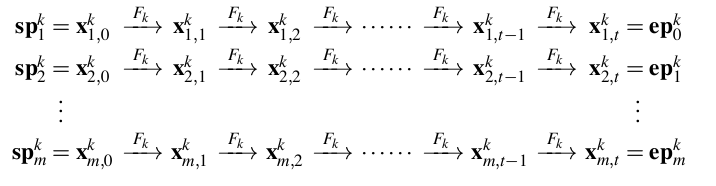
\includegraphics[width=\textwidth]{figures/HellmanMatrix.png}
  \centering
  \label{fig:hellmax}
\end{figure}

Here the starting points are $sp$ they are equal to $x$ which is the first element of the chain. It is then encrypted with the current encryption scheme and the reduction function is applied. This is done $t$ times and then $e_t$ is the endpoint.

\begin{figure}[th]
  \centering
  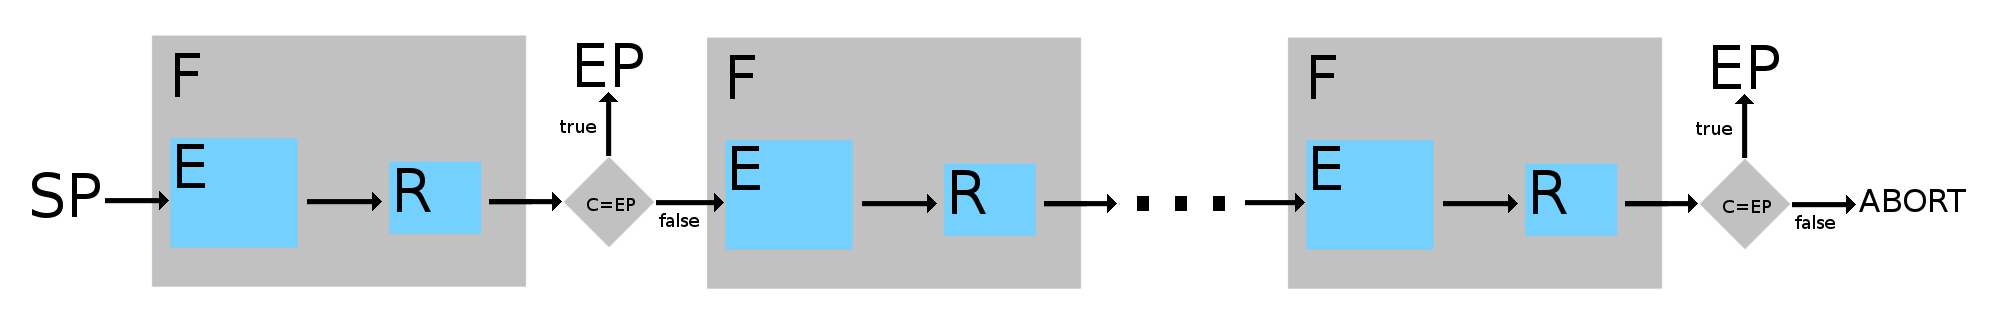
\includegraphics[width=\textwidth]{figures/DPSchema.png}
  \caption{Needs to be changed to Hellman schema}
  \label{fig:hellSchema}
\end{figure}

Each row/chain from \ref{hellmax} is built the way shown in \ref{fig:hellSchema}. When a table is generated it should contain $m$ tuples of (SP,EP) and every chain should contain $t+1$ keys which results in $m\cdot(t+1)$ keys. This should mean that our tables coverage should be m x t, this is not always the case due to merges.

\subsubsection{Merges}
Merges occur when in some point of the generation of two chains, they have the same intermediate point/chain link which causes a collision and  forces the chains merge. This is usually caused by the reduction function, if the reduction function reduces the bit-size of the ciphertext. Say we have ciphertext1 12345678 and ciphertext2 12345679 each of them are 32 bits but as our encryption only takes 28 bits then applying the reduction function to this would cause a merge since the reduction function would remove the last 4 bit. If this was the case the chains would now have merged and all the following intermediate points(chains links) will be the same. This affects the overall coverage of the table, if the merge happens 10 steps into the chain the coverage will have $10 - t$ less keys as the rest of the two chains are duplicates.
\\
illustration of merges
\subsubsection{Loops}
Loops occur when a intermediate point(chain link) points back to a previously reached chain link. This will also result in ad decline of the table coverage.

TODO figure for chain looping

A loop will loop around in the same chain links until it reaches t.

\subsubsection{Multiple Tables}
In Hellman as m and t increases it will reach a point where the coverage will not increase due to merges and loops. This has been calculated to be somewhere near $N^{\frac{2}{3}}$ for single tables \cite{176}. A clever way to increase the success rate and coverage rate for the Hellman trade-off is by adding multiple tables.

\subsection{Online phase}
Once a table is generated and we have a matching text ciphertext pair $(y=F(x))$ the online phase can commence.\\
The given ciphertext is used as the key for the encryption and we compute a single chain. This is done for $1<k<l$ the same way as shown in \ref{fig:hellSchema} each link computed is matched with the computed Hellman table. If it reaches to the last chain link and a match is not found the algorithm will report failure.\\

Whenever a match is found the corresponding SP is returned. The chain is now partially regenerated to obtain $X_{tmp}=x^k_{i,t-j}=F^{t-j}_k(sp^k_i)$. Which should be the key the text was encrypted with:
\begin{equation}
    F^j_k(x_{tmp})=F^j_k(F^(t-j)_k(sp^k_i))=ep^k_i=y^k_j=F^{j-1}_k(y_1)=F^j_k(x)
\end{equation}
\subsubsection{False Alarms}
False alarms happen when in the online phase a match is found, but the
chain did not contain a valid key. This can happen when a merge has
happened earlier when two different chains point to the same end
point. The upper bound for false alarms in a table is $\frac{H_{msc}}{2}$

\subsection{Analysis}
This section will address the success probability, cost of resolving alarms, trade-off curve, memory usage, pre-computational time and online time.

\subsubsection*{Success probability}
The success probability of the table is found by calculating how many keys that are covered in our table. Increasing the size of the table will increase the probability that the key is in it. The amount of keys that are covered depends on the amount of start points and the size of each chain. The success ratio of a single table can be calculated the following way:\\
Lower bound from hellman paper\cite{176}
$\frac{|HM|}{N}>=\frac{1}{N}\sum^{t}_{j=1}\sum^{m}_{i=1}(1-\frac{it}{N})^{j} $
When the all the tables are processed and assuming the reduction functions provide independent results the success probability becomes:
\[1-(1-\frac{|HM|}{N})^l\approx 1- exp(-\frac{l|HM|}{N})\]
Since the count of duplicates is maintained by the matrix stopping rule, the size of the table is :$|HM|\approx mt$.
\subsubsection{Cost of resolving alarms}
The cost of resolving alarms are the following:
\begin{equation}
\text{(cost of resolving alarms for all tables)}>=\frac{H_{msc}}{6}lt
\end{equation}
proof found in \cite{176}
\begin{equation}
\text{(expected cost of resolving alarms)}=\frac{H_{msc}}{6}t
\end{equation}
proof found in \cite{176}
\subsubsection{Trade-off curve}
The trade-off curve can be found by applying the matrix stopping rule to M and T.
\begin{equation}
TM^2\approx N^2
\end{equation}
$T=t \cdot l$ and $M=m\cdot l$
Once the table has been generated it will use M memory and the online phase will take T time.

TODO More on trade-off curves

\subsubsection{Memory Usage}
Storing the table of a TMTO attack such as the Hellman trade-off takes a lot of space. Therefore it is one of the aspects of the time memory trade-off to lower the memory cost to a manageable size. The Hellman trade-off stores a tuple of a start point and a end point this can be described as $m\cdot mem$ where mem is the bit size of the  tuple stored. When several tables are used it is multiplied to the previous equation which gives:
\begin{equation}
M=m\cdot l \cdot mem
\end{equation}
where $l$ is amount of tables.
\subsubsection{Precomputational time}
Time spent on generating the tables are also a factor of the trade-off
curve, the shorter the chains the less time it takes to generate a table. There are m different start points and each of them has t chains, this means that we will use $t\cdot m$ encryptions per table. If $l$ tables are generated the formula for the Time the pre-computation takes is:
\begin{equation}
  Time=m\cdot t\cdot l
\end{equation}
Time is the amount of encryptions that will take place in the generation of the table. Therefore the real world time is Time divided by the amount of encryptions can be done pr second.

\subsubsection{Online time}
Online time is the time it takes to find a key in the worst case scenario. When searching for a key the worst case scenario is when it takes t applications of F, that is to search through the entire table. If the tradeoff consists of more than one table it is again multiplied by the amount of tables $l$.
\begin{equation}
  Time=t\cdot l
\end{equation}
The online phase is also multiplied by the time it takes one encryption or divided by the amount of encryptions per second. A major problem in the online phase of the  Hellman tradeoff is the amount of lookups needed. Even if it is possible to compute a million encryptions per second we need the capacity to access our table a million times pr second. And as our table will be stored on the harddrive it will be impossibru.



\section{Distinguished Points}
\label{sec:dptheory}

The distinguished points - trade-off was first described by Rivest in
the paper [ref] and was further analysed in \cite{DP}. It is a simple modification of the Hellman tradeoff
where one does not have chains of the same size. Instead when a
distinguished point is reached the chain does not continue. The way we distinguish a point is by some property(hence property) (eg. the first 16 bits are zero \code{dp=00001234, dp!=12345678}).Utilizing this, the amount of table lookups in the DP-trade-off is lowered dramatically, since a lookup only happens when a point that matches the property is found.
\subsection{Pre-computational phase}
The online phase of the DP-trade-off is very similar to the Hellman method.
\subsubsection{Parameters}
There are several parameters that decide the size and the coverage of
the DP-tradeoff. M is the amount of rows, t is the chain length  and l is the amount of tables.
To prevent chains from growing uncontrollably $t_{max}$ is used. This is the max size a chain can get before it is aborted and the chain discarded.
Like the Hellman tradeoff the table must satisfy the
given matrix stopping rule $mt^2\approx N$ again the difference between
mt and N should not be too large or to close to zero. Again a
matrixstopping constant is used to hold the difference $mt^2\approx
D_{msc}N$. Reduction functions are selected.... add more. The dp property is given by a bitmask with length $dp_l$.
Once the Parameters have been selected the algorithm can start. $F(SP)=C_1$ is computed and the reduction function is applied which gives the first chain link.$C_1$ is compared to the Dp property, if it is a positive match $C_1$ is an EP this is stored with the SP and the chain length $t_{DP}$. If $C_1$ does not match up with the dp property $F(C_1)=C_2$ is computed and the result compared to the dp property this is done untill an EP is found or the chain length reaches $t_{max}$
\begin{figure}[th]
  DP schema
  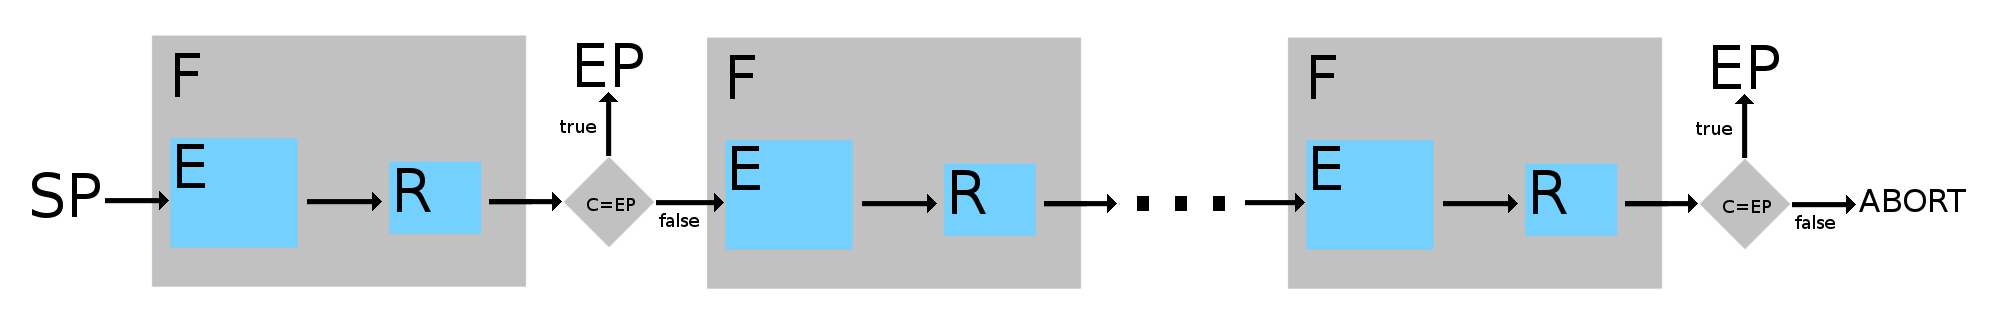
\includegraphics[width=\textwidth]{figures/DPSchema.png}
  \centering
\end{figure}
\subsection{Online phase}
The online phase for the DP-trade-off is also similar to the Hellman-tradeoff online phase. The major difference is that all EP in the computed table are distinguished points therefore instead of checking all chain links that the given ciphertext gives we only check it when a DP is reached. F is applied to C until a DP is reached or it has been applied $t_{max}-1$ times. If it reaches $t_{max}-1$ the key is not covered in the table but if it is reached we check the table for the distinguished point/EP when found we regenerate the chain from the stored SP, Just like in the Hellman tradeoff. When resolving false alarms we we either have to regenerate the entire chain untill the EP is reached. This can be prevented by storing the size of each chain in the table, this wil in turn cause the table size to increase.

\subsection{Analysis}
\subsubsection{DP Property}
The property influences the success rate, coverage, precomputation and online time. This means that the property cannot be selected arbitrarily and needs consideration. If the property requirenment is too easily met the length of each chain will decrease, which will lead to less coverage since less unique keys will be generated. If it is too hard to meet the chains will become larger but there will be less chains since some will be discarded if a point is not found. Which leads to lower coverage and a longer precomputation time. As stated the length of the dp property matters and influences the coverage and thereby the success rate of a table and can therefore neither be too large or too short. Too long chains are stored to rarely and too short chains do not consist of enough unique chain links.

The property also influences the amount of table accesses. In the online phase a chain is generated until i reaches a chain link where the property is met. The probability of finding a match is the following:
\begin{equation}
t(1-e^{-\hat{t}/t})
\end{equation}

\subsubsection{Success Ratio}
The success ratio for the DP trade-off is given by
\begin{equation}
  D_{ps}=1-e^{-D_{cr}D_{pc}}
\end{equation}
Where $D_{cr}$ is the coverage rate and $D_{pc}$ the pre-computational coefficient. Which are found by:
\begin{equation}
  D_{pc}=\frac{mtl}{N}
\end{equation}
\begin{equation}
  D_{cr}=\frac{2}{\sqrt{1+2D_{msc}}+1}
\end{equation}
When $\hat{t}$ is sufficiently large. This is when almost all chains become distinguished points. For $\hat{t}$ to be sufficiently large it should be larger than $t$ but the approximation $(1-\frac{1}{t})^{\hat{t}}\approx e^{-\hat{t}/t}$ should still remain valid.
\subsubsection{Memory Usage}
This will only cover for when $\hat{t}$ is sufficiently large.
The memory usage of the distinguished points depends on the generated table. It depends on the amount of start points, m and the bitwise size of the tuple of (SP, EP) mem and the amounts of tables generated $l$.

\begin{equation}
  M=m\cdot l \cdot mem
\end{equation}

\subsubsection{Precomputation Time}
This will only cover for when $\hat{t}$ is sufficiently large.
Due to the fact that the DP-tradeoff has no fixed chain length each chain takes an individual amount of time when constructed. And it is not allways that the chain is stored, in this case $t_{max}-1$ applications of F has been done for nothing.

\begin{equation}
  insert formula
\end{equation}

\subsubsection{Online Time}
This will only cover for when $\hat{t}$ is sufficiently large.
The online phase for distinguished points is similar to the Hellman
online phase. The length of the initial online chain computed is the
average of the length of chains in the tables L. The online time can
then be described as
\begin{equation}
  Time=L\cdot l
\end{equation}
The amount of table accesses is where the Distinguished points method really shines since in the worst case it will only do one access per table, and best case only one lookup once a point where the dp property holds has been found.

\section{Rainbow Tables}
\label{sec:raintheory}

The last type of dictionary attack we will explore, is the rainbow
attack. The rainbow attack was introduced to improve on the previous
attacks by eliminating the problem of merging chains. In a rainbow
attack the only way a chain can merge, is when a collision happens in
the same row of two pre-computational chains. As the rainbow attack uses different
reduction functions for each row of the chain, collisions happening
any other place will simply continue with different reduction
functions.

Because of this property rainbow tables will also be loop free. This
will save a lot of work compared to the two other discussed attacks.

For the rainbow attack, we will consider tables with $m$ entries build
from $t$-long pre-computational chains. The parameters $m$ and $t$
will be set such that an attack on a cryptographic
function with key size \textbf{N}, will satisfy the matrix
stopping rule $m \cdot t \approx \textbf{N}$. A matrix stopping $R_{msc}$
constant is introduced which will fulfill $m\cdot t = R_{msc} \cdot
\textbf{N}$. Another big difference between the rainbow attack and the
other discussed attacks is the small number of tables $l$, often only
one large table. As for our calculations we will mostly be looking at
rainbow attacks with only one table if nothing else is stated.

\subsection{Pre-computation Phase}

A Rainbow table is built with $m$ entries of end points, where each endpoint
$ep$ in the table is computed by a $t$ long pre-computational chain.

Each endpoint of a row is computed from a chosen/randomly chosen
start point $sp$. From the start point $sp$ the pre-computational chain,
which generates our endpoint, is computed.

For Rainbow tables, the main difference compared to the other
discussed TMTO-attacks is the reduction function. Rainbow attacks
uses $t$ different reduction functions $R_1,R_2..R_t$ to compute a pre-computation
chain of length $t$.

See \ref{fig:rainbowchain} for the structure of an $i$-th
pre-computational chain of a rainbow table.

\begin{figure}[H]
  \centering
  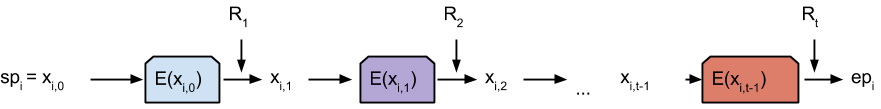
\includegraphics[scale=0.4]{figures/rainbowchain.png}
  \caption{Rainbow Chain - shows weirdly in report Fix?}
  \label{fig:rainbowchain}
\end{figure}

A full rainbow table consists of $m$ iterations of the rainbow chains
with $m$ different starting points.

If no other means of storage optimization is done each chains
starting point and ending point is stored in the rainbow table.

The pre-computation phase of a rainbow attack requires
$R_{msc} \cdot \textbf{N} \cdot l$ calls to the cryptographic function the attack targets.

\subsection{Online phase}
\label{sec:onlinerb}

The online phase of the rainbow attack differs from the other
discussed TMTO attacks, as $t$ reduction functions are used to
generate the table. To look up a key in the rainbow table one has to
compute the online chain for an input $c$. The first element of
the online chain is computed by $R_t(c)$ and looked for in the
table. If no match is found the next element $R_t(f(R_{t-1}(c)))$ is
computed and checked for a match. If nothing is found then $R_t(f(R_{t-1}(f(R_{t-2}(c)))))$
and so on. If an endpoint is found, the chain is reconstructed from the corresponding start
point. If the key is not found in the recounstructed chain it will count
as a false alarm. If the key is found the attack was a
success. This type of table lookup will leave us with at most
$\frac{t(t - 1)}{2}$ calculations of the cryptographic function and
$t$ lookups in the the table.

TODO Figure

\subsection{Analysis}

TODO Same as the other?



%%% Local Variables:
%%% mode: latex
%%% TeX-master: "Thesis"
%%% End:

\chapter{Parameter and table choice}
\label{ch:param}
For the Time-Memory trade-off attack to viable, the right set of
parameters and the right table choice is of huge importance. In this
attack we would ideally want to perform the online phase of the  attack on a modern
high-end laptop/desktop machine. For this to be possible, the right
trade-off between time and memory is needed. For an attack on the
cipher with \code{64-bit} key size, we know a large table is required. But if
we want to make it possible to perform the attack on a (heavily
upgraded) consumer
machine, we need to set an upper bound for the maximal memory
usage. In our attack, we set an upper bound of memory usage to around
\code{8TB} of tables[cite available hd sizes]. We see this as a possible amount of storage if a
consumer machine with a TMTO-attack in mind was to be build.

Knowing this and taking the theory behind the
TMTO-attack\footnote{Chapter \ref{ch:tmto}} into consideration, we
have to argue that this upper bound is required to be hit. For every
trade-off we take towards lower memory usage, the online phase of the
attacks will take a hit.

Another thing to take into consideration when analyzing the parameter
choice and time consumption of the different phases is the table lookup
time. Since generated TMTO tables for a \code{64-bit} key size will
always be larger than a given built machines amount of RAM, look-ups are
done directly on a HDD or SSD. Estimates of how much time is required
for each lookup in a table is hard to do, but will be further analyzed
in SOMEWHERE?

As for success probability of the
the different attacks, we went with $P = 73\%$ as an acceptable
success rate.
We witnessed that for a probability of above $73\%$ the increase,
in both pre-computational cost and the time of the online phase, would
make our initial idea of running the attack on a consumer made PC
unfeasible.

In the following sections we will go through our computations of
parameters for the different TMTO-attacks with these limits set.

\section{Hellman Table}
All calculations of parameters follows the theory provided in \ref{sec:hmtheory}.
Concidering the theory and above mentioned formulas, a approximation of the best parameters for a $73\%$ success rate table can be made.
As stated earlier the memory requirements below $8tb\approx2^{45.863}bit$. First of we can find parameters that fit within those restraints.
As the success probability already is set we can from this find the respective parameters and compare them.

\begin{figure}[H]
  \centering
  \begin{minipage}{0.45\textwidth}
    \centering
    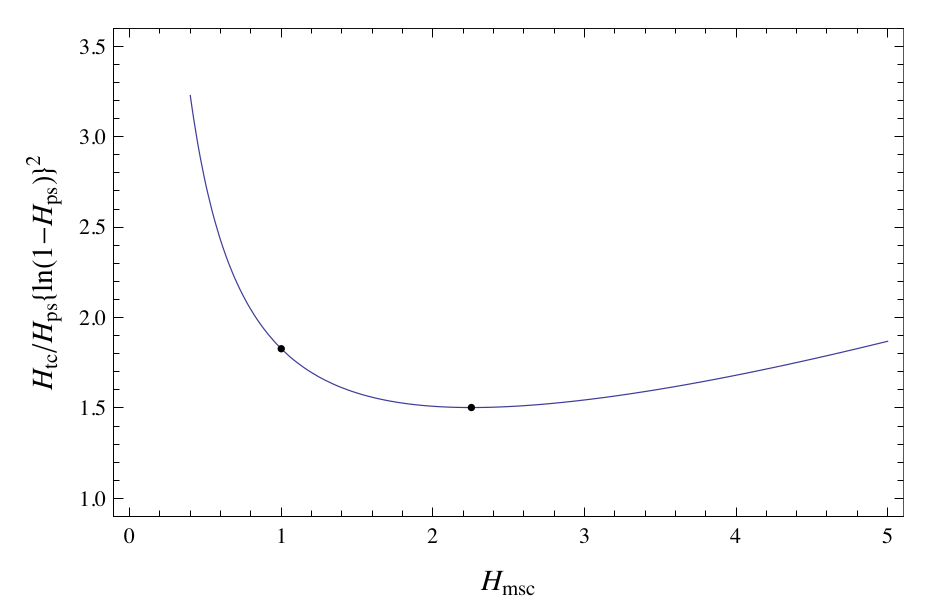
\includegraphics[width=1.2\textwidth]{figures/HellmanTradeOff.png}
    \captionof{figure}{Figure from \cite{176}}
    \label{fig:hellTC}
  \end{minipage}\hfill
  \begin{minipage}{0.45\textwidth}
    \centering
    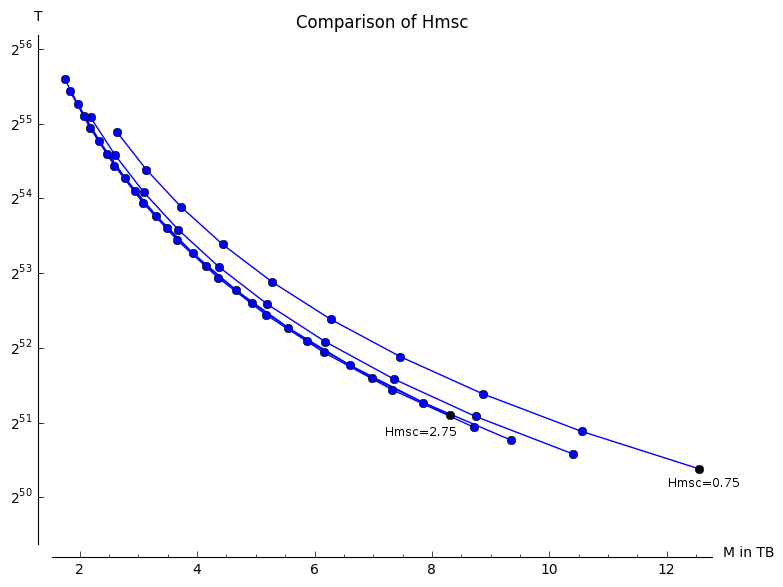
\includegraphics[width=1.2\textwidth]{figures/compareHmsc.png}
    \captionof{figure}{$H_{msc}$ from 0.75 to 2.75}
    \label{fig:hellHmsc}
  \end{minipage}
\end{figure}
The lower a tradeoff coefficient is the better the trade off between memory and time is. Figure \ref{fig:hellTC} is a graph of the tradeoff coefficient for a set success ratio and $H_{msc}$. $H_{msc}$ should be between 1 and 2.25 as seen on the graph\cite{176}. This is further shown in \ref{fig:hellHmsc}, where as $H_{msc}$ grows the smaller the table gets but this effect works with less effect with higher $H_{msc}$. The downside and the reason that the $H_{msc}$ should not be as big as possible is that it influences the precomputation cost and the efficiency of the tradeoff. The optimal value must be where the efficeincy is at its best therefore $H_{msc}$ is $2.25$.
Now to select $m$ $t$ and $l$ from \ref{tab:hellparam}.
\begin{table}[H]
  \centering
  \text{\texttt{Success{ }={ }0.73,{ }Hmsc{ }={ }2.25,{ }Hcr{ }={ }0.74,{ }Htc{ }={ }1.88{ }Hpc{ }={ }1.77} }
\begin{tabular}{lllll}
m & t & l & M in TB & T \\\hline
$2^{10.00}$ & $2^{27.58}$ & $2^{26.63}$ & $1.70$ & $2^{54.10}$ \\
$2^{10.50}$ & $2^{27.33}$ & $2^{26.38}$ & $2.02$ & $2^{53.60}$ \\
$2^{11.00}$ & $2^{27.08}$ & $2^{26.13}$ & $2.41$ & $2^{53.10}$ \\
$2^{11.50}$ & $2^{26.83}$ & $2^{25.88}$ & $2.86$ & $2^{52.60}$ \\
$2^{12.00}$ & $2^{26.58}$ & $2^{25.63}$ & $3.40$ & $2^{52.10}$ \\
$2^{12.50}$ & $2^{26.33}$ & $2^{25.38}$ & $4.05$ & $2^{51.60}$ \\
$2^{13.00}$ & $2^{26.08}$ & $2^{25.13}$ & $4.81$ & $2^{51.10}$ \\
$2^{13.50}$ & $2^{25.83}$ & $2^{24.88}$ & $5.72$ & $2^{50.60}$ \\
$2^{14.00}$ & $2^{25.58}$ & $2^{24.63}$ & $6.81$ & $2^{50.10}$ \\
$2^{14.50}$ & $2^{25.33}$ & $2^{24.38}$ & $8.09$ & $2^{49.60}$ \\
\end{tabular}
  \caption{Hellman Parameters}
  \label{tab:hellparam}
\end{table}


\section{Distinguished Points Table}
$\*$Needs more work$\*$
For this section we assume that $\hat{t}$ is sufficiently large.
All calculations of parameters follows the theory provided in \ref{sec:dptheory}.
Yet again the upper bound for the memory is set to  $8tb\approx2^{45.8}bit$, the success rate has been set as $73\%$. This is the basis for the parameters that will be selected.
As shown in \ref{fig:dpHmsc} the smaller the matrix stopping constant gets the bigger the table gets, The time memory coefficient is most efficient at 0.56 \cite{176}. Which also states that a $D_{msc}$ above 0.56 should be avoided.
Therefore the matrix stopping constant has been set to 0.56, using the formulas for optimal parameters from \cite{176} \ref{tab:DPparam} is generated.
\begin{figure}[H]
  \centering
  need to put lables on the elements from left to right 0.2, 0.3, 0.56, 0.75, 1.00, 1.25
    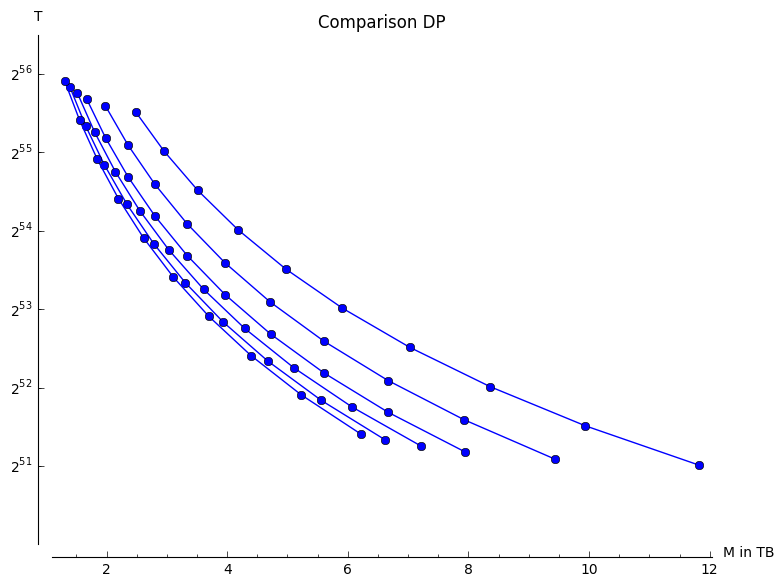
\includegraphics[width=0.5\textwidth]{figures/compareDmsc.png}
    \captionof{figure}{$D_{msc}$ from 0.2 to 1}
    \label{fig:dpHmsc}
\end{figure}
\begin{table}[H]
  \centering
  \text{\texttt{Success{ }={ }0.73,{ }Dmsc{ }={ }0.56,{ }Dcr{ }={ }0.81,{ }Dtc{ }={ }8.77{ }Dpc{ }={ }1.60} }
\begin{tabular}{lllll}
m & t & l & M in TB & T \\\hline
$2^{10.00}$ & $2^{26.58}$ & $2^{28.10}$ & $2.36$ & $2^{54.69}$ \\
$2^{10.50}$ & $2^{26.33}$ & $2^{27.85}$ & $2.81$ & $2^{54.19}$ \\
$2^{11.00}$ & $2^{26.08}$ & $2^{27.60}$ & $3.34$ & $2^{53.69}$ \\
$2^{11.50}$ & $2^{25.83}$ & $2^{27.35}$ & $3.97$ & $2^{53.19}$ \\
$2^{12.00}$ & $2^{25.58}$ & $2^{27.10}$ & $4.72$ & $2^{52.69}$ \\
$2^{12.50}$ & $2^{25.33}$ & $2^{26.85}$ & $5.61$ & $2^{52.19}$ \\
$2^{13.00}$ & $2^{25.08}$ & $2^{26.60}$ & $6.67$ & $2^{51.69}$ \\
$2^{13.50}$ & $2^{24.83}$ & $2^{26.35}$ & $7.94$ & $2^{51.19}$ \\
$2^{14.00}$ & $2^{24.58}$ & $2^{26.10}$ & $9.44$ & $2^{50.69}$ \\
$2^{14.50}$ & $2^{24.33}$ & $2^{25.85}$ & $11.22$ & $2^{50.19}$ \\
 &  &  &  &  &  \\
\end{tabular}
  \caption{DP Parameters}
  \label{tab:DPparam}
\end{table}


\section{Rainbow Table}
\label{sec:rainbowparam}
For the Rainbow Table TMTO attack, we again set \code{8TB} as the
upper bound for memory consumption.

All calculations of parameters follows the theory provided in
\ref{sec:raintheory}.

Conveniently \cite[Fig.4]{176} shows that with our chosen success rate
$P$ the trade-off effiency is actually lowest when the table count is
set to 1.

In our calculations, we assume a sequential approach is done in the
pre-computational phase. This allows us to remove half of the memory
cost compared to storing both start point and end point.

As we have a chosen success rate $P$ set, \cite[Proposition
29]{176} shows that from a given $P$ we can calculate a lower bound
for $R_{msc}$ as follows
\[R_{ps} = 1 - \left( \frac{2}{2 + R_{msc}}^{2l} \right) \Rightarrow R_{msc} = 2 ((1 - R_{ps})^{-\frac{1}{2l}} - 1)\]
Where $R_{ps}$ is the success probability of a rainbow attack. With
that in mind we can now for different values of $m$ compute the
corresponding $t$ value where the $R_{msc}$ is satisfied.

Table \ref{tab:rainparam} shows the relation between \code{t} and
\code{m} in a Rainbow attack, when the success rate of $73\%$ is set\footnote{Tables for $P = 58\%, P = 73\%, P = 90\%$ and tables $l=1..3$ are generated and can be
found in Appendix \ref{sec:rainbowtab}.}. Figures \ref{fig:param73}
and \ref{fig:time73} shows the graphical representation of the table.

\begin{table}[H]
  \centering
  \text{\texttt{Success{ }={ }0.730000,{ }Rmsc{ }={ }1.849002,{ }l{ }={ }1,{ }Offline{ }phase{ }={ }2{\char`\^}64.886747}}
  \begin{tabular}{llll}
    m & t & M(TB) & T \\ \hline
    $2^{35.50}$ & $2^{29.39}$ & $0.39$ & $2^{56.58}$ \\
    $2^{36.00}$ & $2^{28.89}$ & $0.55$ & $2^{55.58}$ \\
    $2^{36.50}$ & $2^{28.39}$ & $0.78$ & $2^{54.58}$ \\
    $2^{37.00}$ & $2^{27.89}$ & $1.10$ & $2^{53.58}$ \\
    $2^{37.50}$ & $2^{27.39}$ & $1.55$ & $2^{52.58}$ \\
    $2^{38.00}$ & $2^{26.89}$ & $2.20$ & $2^{51.58}$ \\
    $2^{38.50}$ & $2^{26.39}$ & $3.11$ & $2^{50.58}$ \\
    $2^{39.00}$ & $2^{25.89}$ & $4.40$ & $2^{49.58}$ \\
    $2^{39.50}$ & $2^{25.39}$ & $6.22$ & $2^{48.58}$ \\
    $2^{40.00}$ & $2^{24.89}$ & $8.80$ & $2^{47.58}$ \\
  \end{tabular}
  \caption{Rainbow Parameters}
  \label{tab:rainparam}
\end{table}
\begin{figure}[H]
  \centering
  \begin{minipage}{.5\textwidth}
    \centering
    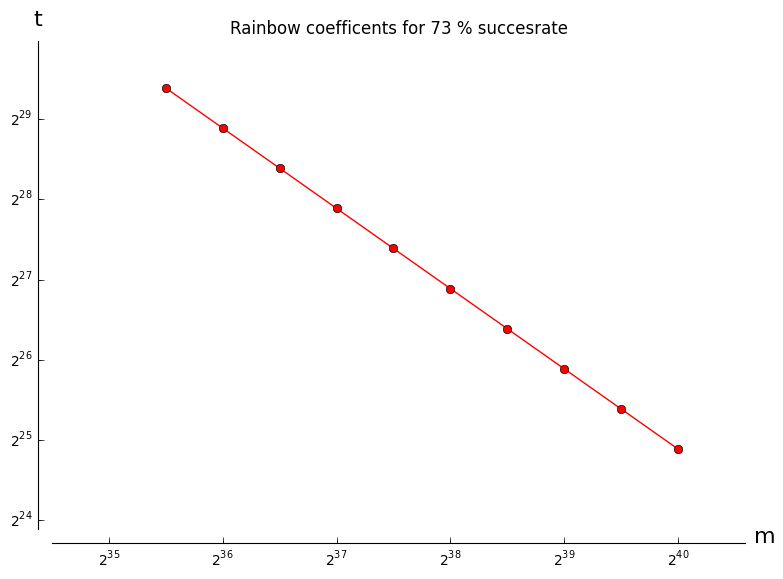
\includegraphics[scale=0.3]{figures/RainbowCoef73.png}
    \captionof{figure}{Rainbow Parameters 73\% success}
    \label{fig:param73}
  \end{minipage}%
  \begin{minipage}{.5\textwidth}
    \centering
    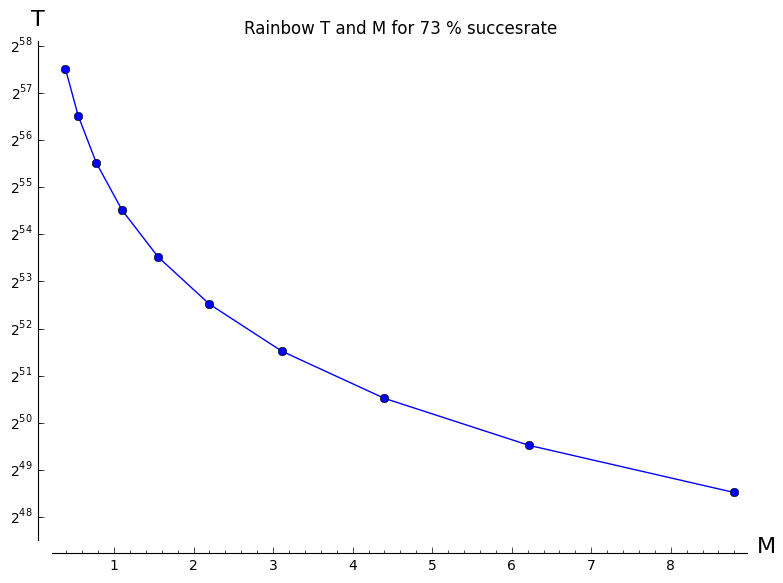
\includegraphics[scale=0.3]{figures/RainbowTime73.png}
    \captionof{figure}{Rainbow TMTO 73\% success}
    \label{fig:time73}
  \end{minipage}
\end{figure}

Looking at table \ref{tab:rainparam} and figures \ref{fig:param73}
and \ref{fig:time73}\footnote{See Appendix \ref{sec:rainbowgraphs} for
  full size graphs} while knowing that

\newpage
\section{Comparison and choice of table}

%%% Local Variables:
%%% mode: latex
%%% TeX-master: "Thesis"
%%% End:

\chapter{Implementation}
\section{KASUMI Cipher}
\subsection{Implementation}
The implemenation of the KASUMI follows the theory described in the
chapter \nameref{ch:kas}.


\subsection{Benchmarks and Performance}
The benchmarks of the KASUMI cipher implemented is performed on two
laptops. The Laptops will each compute the encryption on 64-bit of
data 10.000.000 times. An average time of ten runs of this test is
chosen as the result. Both machines run on Intels Hashwell
architecture with Core i7 CPUs. The specifications of the laptops are as follows:
\begin{table}[h!]
    \begin{tabular}{l|l|l}
                                    & Zenbook - i7           & Yoga
                                                               pro 2 -
      i7\\ \hline
    CPU Frequency                   & 1,8 GHZ @ 2.9ghz TURBO & 2,0 GHZ @ 3.0ghz TURBO \\ \hline
    CPU Cycles/s                    & 2900000000             & 3000000000             \\ \hline
    Times encryption of 64 bit data & 10000000               & 10000000               \\ \hline
    Total bit encyrpted             & 640000000              & 640000000              \\
    \end{tabular}
    \caption{CPU Specs of laptops performing benchmarks}
    \label{tab:specs}
\end{table}\\
The tests will be performed with the
GCC-compiler \footnote{The Gnu Compiler Collection -
  https://gcc.gnu.org/}. They will be performed with different compile
flags for optimization, consisting of no flags, O2, O3 and Ofast as
these are the most common flags for optimization. The two tables
\ref{tab:zen} and \ref{tab:yoga} will show the results of the KASUMI
tests.
\begin{table}[h!]
    \begin{tabular}{l|l|l|l|l}
     Zenbook 1.8 ghz.  & ~                     & ~             & ~              & ~               \\
    GCC compile flags. & Time in sec (average) & Cycles in tot & Cycles per bit & Cycles per byte \\ \hline
    None               & 7,2322                & 20973380000   & 32,77090625    & 262,16725       \\ \hline
    O2                 & 2,0035                & 5810150000    & 9,078359375    & 72,626875       \\ \hline
    O3                 & 1,8945                & 5494050000    & 8,584453125    & 68,675625       \\ \hline
    Ofast              & 1,897                 & 5501300000    & 8,59578125     & 68,76625        \\
    \end{tabular}
    \caption{Zenbook i7 benchmarks}
    \label{tab:zen}
\end{table}
\begin{table}[h!]
    \begin{tabular}{l|l|l|l|l}
     Yoga 2 pro 2.0 ghz. & ~                     & ~             & ~              & ~               \\
    GCC compile flags.   & Time in sec (average) & Cycles in tot & Cycles per bit & Cycles per byte \\ \hline
    None                 & 6,885                 & 20655000000   & 32,2734375     & 258,1875        \\ \hline
    O2                   & 1,933636364           & 5800909091    & 9,063920455    & 72,51136364     \\ \hline
    O3                   & 1,823333333           & 5470000000    & 8,546875       & 68,375          \\ \hline
    Ofast                & 1,835                 & 5505000000    & 8,6015625      & 68,8125         \\
    \end{tabular}
    \caption{Yoga 2 i7 benchmarks}
    \label{tab:yoga}
\end{table}\\


For analysis of the performance of the cipher, gprof \footnote{GNU
  Profiler - https://sourceware.org/binutils/docs/gprof/} is used to
analyze each function and get a clear idea of which functions might
cause slowdowns. The following output is produced from running the
tests and analyzing with gprof:
\begin{lstlisting}[caption=Gprof output,captionpos=b,label=lst:grpof]
    %   cumulative   self              self     total           
 time   seconds   seconds    calls  ns/call  ns/call  name    
 38.56      0.53     0.53 240000024     2.20     2.20  fi
 23.50      0.85     0.32                             keyschedule
 18.36      1.10     0.25 80000008     3.14     9.75  fo
 12.49      1.27     0.17 80000008     2.14     2.14  fl
  4.41      1.33     0.06                             kasumi_enc
\end{lstlisting}
Note that for getting an somewhat accurate representation of the time usage of
each function, the functions of the cipher cannot be inlined. Thus the
attribute \textit{noinline} must be included for each function. This
takes away some of the optimzations done by the Ofast compile
flag. Not supringsingly it shows that \textit{fi} and
\textit{keyschedule} takes up the most computational
power. Since \textit{fi} is used in every round of the cipher and it
requires lookups in a predefined table for every computation, this
could be seen as expected. As for the keyschedule, it's recalculated
in each encryption and therefore will require a new computation in
each new encryption done. 

If we consider the results of \ref{lst:grpof} and look at both
\ref{tab:zen} and \ref{tab:yoga}, this shows us that for each byte
encrypted around 17 cycles of the CPU is used on generating the
keyschedule. That leaves around 50 cylces remaining for the actual
encryption of a text.

Since most of the actual computations TODO assembly vs C? Find kilder?

Further optimization could be gained by using a different compiler. As
both test machines contain Intels i7 CPUs, noticeable performance
increases could be gained by using a Intel compiler. Tests with the
Intel compiler has not been performed. Kilder?

\section{Tablegenerator}

\section{Online Phase}

\section{Usage}


%%% Local Variables:
%%% mode: latex
%%% TeX-master: "Thesis"
%%% End:

\chapter{Analysis}
\label{ch:anal}

\section{TMTO Attack}
As the keysize of an attack on the KASUMI cipher used in the 2G
network is \code{64-bit}, we have to perform our tests on a scaled down
key. With the hardware at our disposal the computation of a table
required to perform the attack on a \code{64-bit} key would simply be
unrealistic. Therefore all of our testing is done on tables generated
with \code{32-bit} keys. We use the same idea as the scaling from \code{128-bit} to
\code{64-bit} discussed in chapter \ref{ch:kas}.

Thus a key $K$ built from a \code{32-bit} $K_{32} = K_1 || K_2$  implementation will
look as follows
\[K = K_1 || K_2 || K_1 || K_2 || K_1 || K_2 || K_1 || K_2\]
As to gain an idea of how our implementation matches up with
the math and parameter choices done in chapter \ref{ch:param}, we have to generate
information on an actual attack on a \code{32-bit} key. If the \code{32-bit} test
results match with our calculations, we can begin to give estimates
on the actual attack(\code{64-bit} keysize).
\subsection{Pre-computational phase}
To test the table generation we will first set some parameters
valid for \code{32-bit} testing.

Using the same parameter setup as described in \ref{sec:rainbowparam}
table \ref{tab:rainparam32} gives us valid parameter choices. For the
testing of \code{32-bit} no boundaries were set.
\begin{table}[H]
  \centering
  \text{\texttt{Success{ }={ }0.730000,{ }Rmsc{ }={ }1.849002,{ }l{ }={ }1,{ }Offline{ }phase{ }={ }2{\char`\^}32.886747}}
  \begin{tabular}{llll}
    m & t & M(MB) & T \\ \hline
    $2^{25.00}$ & $2^{7.89}$ & $134.22$ & $2^{13.67}$ \\
    $2^{25.50}$ & $2^{7.39}$ & $189.81$ & $2^{12.71}$ \\
    $2^{26.00}$ & $2^{6.89}$ & $268.44$ & $2^{11.76}$ \\
    $2^{26.50}$ & $2^{6.39}$ & $379.63$ & $2^{10.83}$ \\
    $2^{27.00}$ & $2^{5.89}$ & $536.87$ & $2^{9.92}$ \\
  \end{tabular}
  \caption{Rainbow Parameters - 32-bit keysize}
  \label{tab:rainparam32}
\end{table}
Since we are only testing on \code{32-bit} there is no real concern of
memory usage or online time. For this reason we went with a parameter
choice of $m=2^{25} \approx 33445532$ and $t= 2^{7.89} \approx
236$. The table generator will be tested on the actual
pre-computational time and the memory usage.

\textbf{Pre-computational time}

Table \ref{tab:rainparam32} states that an expected amount of
KASUMI encryptions required for generation of the table is
$2^{32.886}$. Looking back to \ref{sec:benchkas} we know the
amount of time it takes our test machines to perform 10000000 encrytions. As an
example the previously mentioned Zenbook i7 is used. The
Zenbook will perform 10000000 KASUMI encryptions in 1,897
seconds. From this we get an idea of how many encryptions our
machine execute in 1 second.
\[10000000 enc / 1.897 s = 5291005,29 \quad enc/s\]
Now we can calculate the expected running time of the
pre-computational phase
\[2^{32.886} / 5291005.29 \approx 1500s = 25 min \]
Running our implementation with UNIX-command
\code{time}\footnote{\url{https://en.wikipedia.org/wiki/Time_(Unix)}}
allows us to easily check whether or not this matches up. Running the
implementation multiple times resulted in average running time of
approximately 27 minutes. This is $\approx8\%$ more time used than
expected. This can be seen as expected as time is required to write
the table to a disk. Another explanation could be our sequential
approach and the usage of the MD5 algorithm. TODO Some facts to back up maybe?

\textbf{Memory}

We also want to make sure that the actual memory usage matches up with
the expected. From our parameter choice we can see the expected memory
$M_{predicted}=134.22$MB. The previously generated table can easily be
checked to make sure this is correct. Using the UNIX-command
\code{wc}\footnote{\url{https://en.wikipedia.org/wiki/Wc_(Unix)}} with
the \code{-c} flag will allow us to get the byte count of the
generated binary file. Performing this command on our generated table
unsurprisingly gave us a result of
$M_{actual}=134217728\text{B}\approx134.22$MB.

Knowing the time usage and memory usage in the pre-computational phase
matches up with our expected values, we can now give an approximate of
how scaling from a \code{32-bit} keysize to a \code{64-bit} keysize
will look.

Again we take a look back to \ref{sec:rainbowparam}. As we are now
dealing with the actual \code{64-bit} attack the boundaries we set
will now be taken into account again. From the tests on the
\code{32-bit} implementation we saw the size of the table match up
perfectly. Because of this we will not discuss table size further, as
adding additional bit to a binary file should not change the outcome.
Going with the parameters chosen in \ref{sec:rainbowparam} we set
$m=?$ and $t=?$.

From the chosen parameters we know that the pre-computational phase is
estimated to require $2^{64.88}$ encryptions of KASUMI. This amount of encryptions
is infeasible to test on the devices that we ran the
\code{32-bit} implementation on.

TODO Need to ask Andrey about what we can compare with.. HPC clusters?

\subsection{Online phase}
As stated earlier are the tests preformed on a scaled down version of the keyspace.
The tests are run on the 32 bit implementation and then scaled up.
Firstly the Time it takes is compared to our computations, as Time is found by $Time=\frac{t\cdot(t-1)}{2}$.
Table\ref{tab:OnlineT} shows each of our test tables worst case run times and the calculated encryption time for each of them.
Each  table has an online encryption time spanning from a few miliseconds to a few microseconds, wheras the total time is  much larger.
Furthermore if we don't add in the fact that the computer is smart and caches memory it takes even longer, which is shown in the T lookup field(this the time one lookup takes when it isn't in memory multiplied with t which is the amount of lookups).
\begin{table}[H]
\centering
\caption{Online Time Comparison}
\label{tab:OnlineT}
\begin{tabular}{|c|ccccc}
\hline
Table          & \multicolumn{1}{c|}{t rounded up} & \multicolumn{1}{c|}{Total time} & \multicolumn{1}{c|}{T lookup} & \multicolumn{1}{c|}{T enc} & \multicolumn{1}{c|}{encryptions} \\ \hline
134MB / 73\%   & 236                           & 7.5995 s                        & 7.972375 s                    & 5.24E-03 s                 & 27,730.00                        \\ \cline{1-1}
4300MB / 73\%  & 8                             & 27.339 s                        & 36.724 s                      & 5.29E-06 s                 & 28.00                            \\ \cline{1-1}
8500MB / 73\%  & 4                             & 73.35 s                         & 67.196 s                      & 1.13E-06 s                 & 6.00                             \\ \cline{1-1}
12000MB / 73\% & 3                             & 70.97 s                         & 69.811 s                      & 5.67E-07 s                 & 3.00                             \\ \cline{1-1}
17000MB / 73\%  & 2                             & 66.96 s                         & 65.11 s                       & 1.89E-07 s                 & 1.00                             \\ \cline{1-1}
\end{tabular}
\end{table}
This means that the biggest bottleneck in the implementation is the lookup time. To further investigate this we calculate the lookup time for each table, and compare them to each other note that the test computer has a max read speed of 540 mb/s. One thing we noticed is when the entire table can fit in memory the access time of it increases dramatically, for the 4.3GB table the first table lookup took 4.4 seconds and the lookups afterwards took between 0.6-1 seconds. This is probably due to the table getting cached.
\begin{table}[h]
\centering
\caption{Access time}
\label{tab:memory}
\begin{tabular}{|c|clccc}
\hline
\multicolumn{1}{|l|}{Buffer-size$\downarrow$ Table-size$\rightarrow$}& \multicolumn{1}{c|}{134MB} & \multicolumn{1}{l|}{4300MB} & \multicolumn{1}{c|}{8500MB} & \multicolumn{1}{c|}{12000MB} & \multicolumn{1}{l|}{17000MB} \\ \hline
33554432                                     & 0.0427s                    & 4.4395s                     & 16.829s                     & 23.230s                      & 32.562s                      \\ \cline{1-1}
524288                                       & 0.023s                     & 4.4395s                     & 16.645s                     & 23.279s                      & 32.72s                       \\ \cline{1-1}
65536                                        & 0.021s                     & 4.4585s                     & 16.941s                     & 23.002s                      & 32.483s                      \\ \cline{1-1}
32                                           & 0.053s                     & 5.0245s                     & 16.780s                     & 23.57s                       & 32.44s                       \\ \cline{1-1}
\multicolumn{1}{|l|}{Scaled to 8 tb table}   & 0.6 Hours                  & 2.37 Hours                  & 4.45 Hours                   & 4.31 Hours                   & 4.25 Hours                   \\ \cline{1-1}
\end{tabular}
\end{table}
As \ref{fig:memory} shows the buffer size does not seem to matter much the results fluxuates half a second at most.
The table also shows what the lookup time would be if the table was 8 tb. Where target table size is tts, table size is ts, s is the time one lookup takes in seconds and 3600 is to get it in hours $\frac{\frac{tts}{ts/s}}{3600}$
\begin{figure}[th]
  \centering
  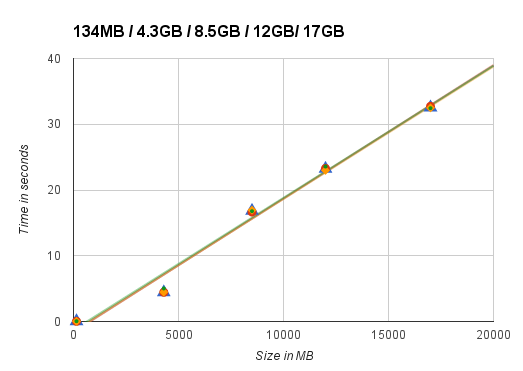
\includegraphics[width=0.8\textwidth]{figures/AccessTime.png}
  \caption{Access time for different table sizes and buffer sizes\\
    Green buffersize= 33554432 bit\\
    Red buffersize = 524288 bit\\
    Orange buffersize = 65536 bit\\
    Blue buffersize = 32 bit\\
    }
  \label{fig:tableAccess}
\end{figure}

Also something to note when scaling the access time up to a table that is 8tb the lookup time is around 4.2-4.45 hours.
One thing to note though is when the table is small enough to fit the memory it gives faster results, which can be ignored since the entire 8 tb table does not fit memory. Now where the access time is estimated we can give a approximation of the online phase for the \code{64-bit} keyspace. As previously stated the access time would lie around 4.2-4.45 hours for each lookup, so for $m=2^{39.80}$ and $t=2^{25.08}$ this means that the lookup time comes to $t\cdot lookupTime=2^{25.08}\cdot 4.45 Hours \approx 18,005 years$. The Encryption time would be $2^{25.08}\cdot\frac{2^{25.08}-1}{2}\approx \frac{6.2897672e+14 encryptions}{5291005 encryptions/sec} \approx 3.7 years$ so the online phase would approximately take $18008.7 years$. Which leads to the conclusion that our implementation would not work in its current state. To get a more realistic attack we will in section \ref{sec:Discussion} explain some memory optimizations and the RainbowDP table that reduces the amount from t to 1. To get the encryption time down to approximately one day one would need 1280 cores.


\section{Cost analysis}
In this section we will assume that the memory optimizations has been implemented and the table is of Rainbow/DP\ref{sec:Discussion}. This gives a table access of 1, when a DP is reached.
To pull this off for $m=2^{39.80}$ and $t=2^{25.08}$ the pre-computation will require \code{7.56TB}, and \code{$2^{64.88}$} encryptions. The online phase will require \code{$2^{49.16}$} encryptions, our cost analysis will aim at getting the online phases encryption time down to one day. This will require $\frac{2^{49.16}}{60*60*24}\approx 2^{32.76}$ encryptions per second. We have found a couple of candidates that fits the bill:

% Please add the following required packages to your document preamble:
% \usepackage[table,xcdraw]{xcolor}
% If you use beamer only pass "xcolor=table" option, i.e. \documentclass[xcolor=table]{beamer}
\begin{table}[h]
\caption{Hardware comparison}
\label{my-label}
\begin{tabular}{|ccccccc}
\hline
\rowcolor[HTML]{EFEFEF}
CPU                                    &                             &                               &                           &                                 &                            & \multicolumn{1}{l|}{\cellcolor[HTML]{EFEFEF}} \\ \hline
\multicolumn{1}{|c|}{Model}            & \multicolumn{1}{c|}{Cores}   & \multicolumn{1}{c|}{Amount} & \multicolumn{1}{c|}{Ghz}  & \multicolumn{1}{c|}{Enc per sec} & \multicolumn{1}{c|}{Price USD} & \multicolumn{1}{c|}{Total USD}                    \\ \hline
\multicolumn{1}{|l|}{AMD FX-8320}      & 8                            & 143                         & 3,5                       & 7278941245                      & 139                    & 20020                                     \\
\multicolumn{1}{|l|}{AMD FX-8350}      & 8                            & 125                         & 4                         & 7271669575                      & 170                   & 21250                                    \\ \hline
\rowcolor[HTML]{EFEFEF}
Hard Drive                                                          &                               &                           &                                 &                           & & \multicolumn{1}{l|}{\cellcolor[HTML]{EFEFEF}} \\ \hline
\multicolumn{1}{|c|}{Model}            & \multicolumn{1}{c|}{Size GB} & \multicolumn{1}{c|}{Amount} & \multicolumn{1}{c|}{Read $mb/s$} & \multicolumn{1}{c|}{Write $mb/s$}      & \multicolumn{1}{c|}{Price USD} & \multicolumn{1}{c|}{Total USD}                    \\ \hline
\multicolumn{1}{|c|}{Crucial}          & 960                          & 8                           & 500                       & 400                             & 300                        & 2400                                          \\
\multicolumn{1}{|c|}{Mushkin} & 1000                         & 8                            & 560                       & 460                             & 339                        & 2712                                          \\ \cline{1-1}
\end{tabular}
\end{table}
So with around $20020+2712=22732 $USD $ \approx 151313 $DK for the harddrive and the CPU's.

%%% Local Variables:
%%% mode: latex
%%% TeX-master: "Thesis"
%%% End:

\chapter{Discussion}
\label{ch:disc}
%%% Local Variables:
%%% mode: latex
%%% TeX-master: "Thesis"
%%% End:

\chapter{Conclusion}
\label{ch:concl}
A summary of the main part of the text
A deduction made on the basis of the main body
Your personal opinion on what has been discussed
A statement about the limitations of the work
A comment about the future based on what has been discussed
The implications of the work for future research

In this project we tried to analyze a practical attack on the KASUMI
block cipher by implementing a time-memory trade-off attack. We
conducted experiments to determine whether or not this attack can be
seen as practical. 

The biggest obstacle in performing this attack will undoubtedly be
computation of the tables needed for the attack. Generating such table
will require more than $2^{64}$ computations of KASUMI if a decent
success probability is expected.

Our implementation of the attack is also very unoptimized when
considering large tables consisting of multiple terabytes of
data. Read times and lookups in tables will prove to be a huge
hindrance if the attack is to be performed on the full keyspace of
\code{64-bit}.

If the attack is to be considered doable the combined approach of 
rainbow and DP attacks should definitely a part of the
implementation. 

%%% Local Variables:
%%% mode: latex
%%% TeX-master: "Thesis"
%%% End:

\appendix
\chapter{Appendix}
\section{Installation}
\label{sec:inst}
Get the source:

\quad\code{\$ git clone \url{https://github.com/kiaer/kasumi.git}}

Build the TMTO-attack. This will generate the executable
\code{bin/tmto}

\quad\code{\$ make }

The executable \code{tmto} can now be executed with an appropriate
flag:

\quad\code{\$ ./bin/tmto [command]}

The following commands is available to use with \code{tmto}:
\begin{verbatim}
usage: ./bin/tmto [command] 
                -t      Generates 32-bit Rainbow Table 
                -o      Performs online phase on 32-bit Rainbow Table 
                -b      Generates 64-bit Rainbow Table 
                -k      Performs online phase on 64-bit Rainbow Table 
                -h      Prints the very helpful usage message.. 
\end{verbatim}

Generating a table for either the 32-bit or the 64-bit key, the table
is stored in the kasumi root folder as either \code{table32.bin} or
\code{table64.bin}. The onlinephase will perform the attack on its
respective table.

Generation of the cipher, for test purposes is also possible:

\quad\code{\$ make cipher}

An executable \code{bin/kasumi\_test} is created. 

%%% Local Variables:
%%% mode: latex
%%% TeX-master: "Thesis"
%%% End:
                                 %Appendix A
\chapter{Graphs and Tables}
\section{Hellman Table Parameters}
\begin{table}[H]
  \centering
  \text{\texttt{Success{ }={ }0.58,{ }Hmsc{ }={ }1,{ }Hcr{ }={ }0.86,{ }Htc{ }={ }0.78{ }Hpc{ }={ }1} }
\begin{tabular}{lllll}
m & t & l & M in TB & T \\\hline
$2^{10.00}$ & $2^{27.00}$ & $2^{27.00}$ & $2.20$ & $2^{53.64}$ \\
$2^{10.50}$ & $2^{26.75}$ & $2^{26.75}$ & $2.61$ & $2^{53.14}$ \\
$2^{11.00}$ & $2^{26.50}$ & $2^{26.50}$ & $3.11$ & $2^{52.64}$ \\
$2^{11.50}$ & $2^{26.25}$ & $2^{26.25}$ & $3.69$ & $2^{52.14}$ \\
$2^{12.00}$ & $2^{26.00}$ & $2^{26.00}$ & $4.39$ & $2^{51.64}$ \\
$2^{12.50}$ & $2^{25.75}$ & $2^{25.75}$ & $5.22$ & $2^{51.14}$ \\
$2^{13.00}$ & $2^{25.50}$ & $2^{25.50}$ & $6.21$ & $2^{50.64}$ \\
$2^{13.50}$ & $2^{25.25}$ & $2^{25.25}$ & $7.39$ & $2^{50.14}$ \\
$2^{14.00}$ & $2^{25.00}$ & $2^{25.00}$ & $8.78$ & $2^{49.64}$ \\
$2^{14.50}$ & $2^{24.75}$ & $2^{24.75}$ & $10.45$ & $2^{49.14}$ \\
\end{tabular}
\caption{Hellman Parameters for $58\%$ $Hmsc = 1$}
\end{table}
\begin{table}[H]
  \centering
  \text{\texttt{Success{ }={ }0.73,{ }Hmsc{ }={ }1,{ }Hcr{ }={ }0.86,{ }Htc{ }={ }2.29{ }Hpc{ }={ }1.52} }
\begin{tabular}{lllll}
m & t & l & M in TB & T \\\hline
$2^{9.00}$ & $2^{27.50}$ & $2^{28.10}$ & $2.36$ & $2^{54.98}$ \\
$2^{9.50}$ & $2^{27.25}$ & $2^{27.85}$ & $2.81$ & $2^{54.48}$ \\
$2^{10.00}$ & $2^{27.00}$ & $2^{27.60}$ & $3.34$ & $2^{53.98}$ \\
$2^{10.50}$ & $2^{26.75}$ & $2^{27.35}$ & $3.98$ & $2^{53.48}$ \\
$2^{11.00}$ & $2^{26.50}$ & $2^{27.10}$ & $4.73$ & $2^{52.98}$ \\
$2^{11.50}$ & $2^{26.25}$ & $2^{26.85}$ & $5.62$ & $2^{52.48}$ \\
$2^{12.00}$ & $2^{26.00}$ & $2^{26.60}$ & $6.69$ & $2^{51.98}$ \\
$2^{12.50}$ & $2^{25.75}$ & $2^{26.35}$ & $7.95$ & $2^{51.48}$ \\
$2^{13.00}$ & $2^{25.50}$ & $2^{26.10}$ & $9.46$ & $2^{50.98}$ \\
$2^{13.50}$ & $2^{25.25}$ & $2^{25.85}$ & $11.25$ & $2^{50.48}$ \\
\end{tabular}
 \caption{Hellman Parameters for $73\%$ $Hmsc = 1$}
\end{table}
\begin{table}[H]
  \centering
  \text{\texttt{Success{ }={ }0.90,{ }Hmsc{ }={ }1,{ }Hcr{ }={ }0.86,{ }Htc{ }={ }8.72{ }Hpc{ }={ }2.67} }
\begin{tabular}{lllll}
m & t & l & M in TB & T \\\hline
$2^{8.00}$ & $2^{28.00}$ & $2^{29.42}$ & $2.94$ & $2^{56.29}$ \\
$2^{8.50}$ & $2^{27.75}$ & $2^{29.17}$ & $3.50$ & $2^{55.79}$ \\
$2^{9.00}$ & $2^{27.50}$ & $2^{28.92}$ & $4.16$ & $2^{55.29}$ \\
$2^{9.50}$ & $2^{27.25}$ & $2^{28.67}$ & $4.94$ & $2^{54.79}$ \\
$2^{10.00}$ & $2^{27.00}$ & $2^{28.42}$ & $5.88$ & $2^{54.29}$ \\
$2^{10.50}$ & $2^{26.75}$ & $2^{28.17}$ & $6.99$ & $2^{53.79}$ \\
$2^{11.00}$ & $2^{26.50}$ & $2^{27.92}$ & $8.32$ & $2^{53.29}$ \\
$2^{11.50}$ & $2^{26.25}$ & $2^{27.67}$ & $9.89$ & $2^{52.79}$ \\
$2^{12.00}$ & $2^{26.00}$ & $2^{27.42}$ & $11.76$ & $2^{52.29}$ \\
$2^{12.50}$ & $2^{25.75}$ & $2^{27.17}$ & $13.99$ & $2^{51.79}$ \\
\end{tabular}
  \caption{Hellman Parameters for $90\%$ $Hmsc = 1$}
\end{table}

\begin{figure}[H]
  \centering
  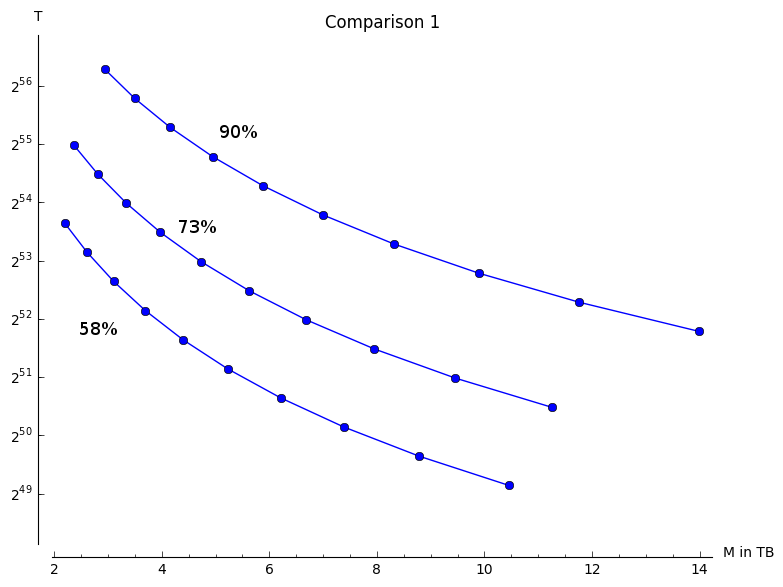
\includegraphics[scale=0.4]{figures/compareHmsc1.png}
  \caption{Comparison of 58\%, 73\% and 90\% success TMTO}
  \label{fig:comparisonhell}
\end{figure}


\begin{table}[H]
  \centering
  \text{\texttt{Success{ }={ }0.58,{ }Hmsc{ }={ }2.25,{ }Hcr{ }={ }0.74,{ }Htc{ }={ }0.64{ }Hpc{ }={ }1.16} }
\begin{tabular}{lllll}
m & t & l & M in TB & T \\\hline
$2^{10.00}$ & $2^{27.58}$ & $2^{26.63}$ & $1.70$ & $2^{54.10}$ \\
$2^{10.50}$ & $2^{27.33}$ & $2^{26.38}$ & $2.02$ & $2^{53.60}$ \\
$2^{11.00}$ & $2^{27.08}$ & $2^{26.13}$ & $2.41$ & $2^{53.10}$ \\
$2^{11.50}$ & $2^{26.83}$ & $2^{25.88}$ & $2.86$ & $2^{52.60}$ \\
$2^{12.00}$ & $2^{26.58}$ & $2^{25.63}$ & $3.40$ & $2^{52.10}$ \\
$2^{12.50}$ & $2^{26.33}$ & $2^{25.38}$ & $4.05$ & $2^{51.60}$ \\
$2^{13.00}$ & $2^{26.08}$ & $2^{25.13}$ & $4.81$ & $2^{51.10}$ \\
$2^{13.50}$ & $2^{25.83}$ & $2^{24.88}$ & $5.72$ & $2^{50.60}$ \\
$2^{14.00}$ & $2^{25.58}$ & $2^{24.63}$ & $6.81$ & $2^{50.10}$ \\
$2^{14.50}$ & $2^{25.33}$ & $2^{24.38}$ & $8.09$ & $2^{49.60}$ \\
\end{tabular}
\caption{Hellman Parameters for $58\%$ $Hmsc = 2.25$}
\end{table}
\begin{table}[H]
  \centering
  \text{\texttt{Success{ }={ }0.73,{ }Hmsc{ }={ }2.25,{ }Hcr{ }={ }0.74,{ }Htc{ }={ }1.88{ }Hpc{ }={ }1.77} }
\begin{tabular}{lllll}
m & t & l & M in TB & T \\\hline
$2^{9.00}$ & $2^{28.08}$ & $2^{27.74}$ & $1.83$ & $2^{55.44}$ \\
$2^{9.50}$ & $2^{27.83}$ & $2^{27.49}$ & $2.18$ & $2^{54.94}$ \\
$2^{10.00}$ & $2^{27.58}$ & $2^{27.24}$ & $2.59$ & $2^{54.44}$ \\
$2^{10.50}$ & $2^{27.33}$ & $2^{26.99}$ & $3.08$ & $2^{53.94}$ \\
$2^{11.00}$ & $2^{27.08}$ & $2^{26.74}$ & $3.66$ & $2^{53.44}$ \\
$2^{11.50}$ & $2^{26.83}$ & $2^{26.49}$ & $4.36$ & $2^{52.94}$ \\
$2^{12.00}$ & $2^{26.58}$ & $2^{26.24}$ & $5.18$ & $2^{52.44}$ \\
$2^{12.50}$ & $2^{26.33}$ & $2^{25.99}$ & $6.16$ & $2^{51.94}$ \\
$2^{13.00}$ & $2^{26.08}$ & $2^{25.74}$ & $7.33$ & $2^{51.44}$ \\
$2^{13.50}$ & $2^{25.83}$ & $2^{25.49}$ & $8.71$ & $2^{50.94}$ \\
\end{tabular}
 \caption{Hellman Parameters for $73\%$ $Hmsc = 2.25$}
\end{table}
\begin{table}[H]
  \centering
  \text{\texttt{Success{ }={ }0.90,{ }Hmsc{ }={ }2.25,{ }Hcr{ }={ }0.74,{ }Htc{ }={ }7.17{ }Hpc{ }={ }3.11} }
\begin{tabular}{lllll}
m & t & l & M in TB & T \\\hline
$2^{8.00}$ & $2^{28.58}$ & $2^{29.05}$ & $2.28$ & $2^{56.74}$ \\
$2^{8.50}$ & $2^{28.33}$ & $2^{28.80}$ & $2.71$ & $2^{56.24}$ \\
$2^{9.00}$ & $2^{28.08}$ & $2^{28.55}$ & $3.22$ & $2^{55.74}$ \\
$2^{9.50}$ & $2^{27.83}$ & $2^{28.30}$ & $3.83$ & $2^{55.24}$ \\
$2^{10.00}$ & $2^{27.58}$ & $2^{28.05}$ & $4.56$ & $2^{54.74}$ \\
$2^{10.50}$ & $2^{27.33}$ & $2^{27.80}$ & $5.42$ & $2^{54.24}$ \\
$2^{11.00}$ & $2^{27.08}$ & $2^{27.55}$ & $6.44$ & $2^{53.74}$ \\
$2^{11.50}$ & $2^{26.83}$ & $2^{27.30}$ & $7.66$ & $2^{53.24}$ \\
$2^{12.00}$ & $2^{26.58}$ & $2^{27.05}$ & $9.11$ & $2^{52.74}$ \\
$2^{12.50}$ & $2^{26.33}$ & $2^{26.80}$ & $10.84$ & $2^{52.24}$ \\
\end{tabular}
  \caption{Hellman Parameters for $90\%$ $Hmsc = 2.25$}
\end{table}

\begin{figure}[H]
  \centering
  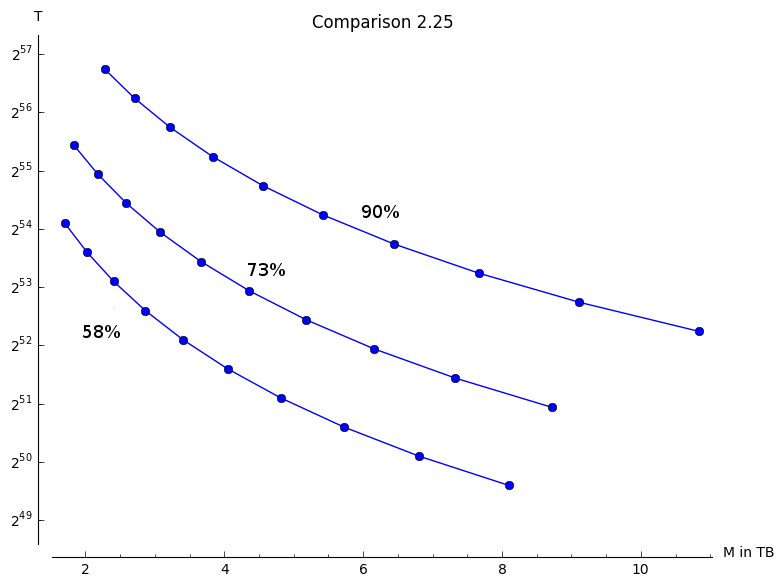
\includegraphics[scale=0.4]{figures/compareHmsc2.25.png}
  \caption{Comparison of 58\%, 73\% and 90\% success TMTO}
  \label{fig:comparisonhell2.25}
\end{figure}

\section{DP table Parameters}
\begin{table}[H]
  \centering
  \text{\texttt{Success{ }={ }0.58,{ }Dmsc{ }={ }0.56,{ }Dcr{ }={ }0.81,{ }Dtc{ }={ }3.53{ }Dpc{ }={ }1.13} }
\begin{tabular}{lllll}
m & t & l & M in TB & T \\\hline
$2^{10.00}$ & $2^{26.58}$ & $2^{27.59}$ & $1.65$ TB & $2^{54.17}$ \\
$2^{10.50}$ & $2^{26.33}$ & $2^{27.34}$ & $1.96$ TB & $2^{53.67}$ \\
$2^{11.00}$ & $2^{26.08}$ & $2^{27.09}$ & $2.34$ TB & $2^{53.17}$ \\
$2^{11.50}$ & $2^{25.83}$ & $2^{26.84}$ & $2.78$ TB & $2^{52.67}$ \\
$2^{12.00}$ & $2^{25.58}$ & $2^{26.59}$ & $3.30$ TB & $2^{52.17}$ \\
$2^{12.50}$ & $2^{25.33}$ & $2^{26.34}$ & $3.93$ TB & $2^{51.67}$ \\
$2^{13.00}$ & $2^{25.08}$ & $2^{26.09}$ & $4.67$ TB & $2^{51.17}$ \\
$2^{13.50}$ & $2^{24.83}$ & $2^{25.84}$ & $5.55$ TB & $2^{50.67}$ \\
$2^{14.00}$ & $2^{24.58}$ & $2^{25.59}$ & $6.60$ TB & $2^{50.17}$ \\
$2^{14.50}$ & $2^{24.33}$ & $2^{25.34}$ & $7.85$ TB & $2^{49.67}$ \\
\end{tabular}
\caption{DP Parameters for $58\%$}
\end{table}
\begin{table}[H]
  \centering
  \text{\texttt{Success{ }={ }0.73,{ }Dmsc{ }={ }0.56,{ }Dcr{ }={ }0.81,{ }Dtc{ }={ }8.77{ }Dpc{ }={ }1.61} }
\begin{tabular}{lllll}
m & t & l & M in TB & T \\\hline
$2^{10.00}$ & $2^{26.58}$ & $2^{28.10}$ & $2.36$ TB & $2^{54.69}$ \\
$2^{10.50}$ & $2^{26.33}$ & $2^{27.85}$ & $2.81$ TB & $2^{54.19}$ \\
$2^{11.00}$ & $2^{26.08}$ & $2^{27.60}$ & $3.34$ TB & $2^{53.69}$ \\
$2^{11.50}$ & $2^{25.83}$ & $2^{27.35}$ & $3.97$ TB & $2^{53.19}$ \\
$2^{12.00}$ & $2^{25.58}$ & $2^{27.10}$ & $4.72$ TB & $2^{52.69}$ \\
$2^{12.50}$ & $2^{25.33}$ & $2^{26.85}$ & $5.61$ TB & $2^{52.19}$ \\
$2^{13.00}$ & $2^{25.08}$ & $2^{26.60}$ & $6.67$ TB & $2^{51.69}$ \\
$2^{13.50}$ & $2^{24.83}$ & $2^{26.35}$ & $7.94$ TB & $2^{51.19}$ \\
$2^{14.00}$ & $2^{24.58}$ & $2^{26.10}$ & $9.44$ TB & $2^{50.69}$ \\
$2^{14.50}$ & $2^{24.33}$ & $2^{25.85}$ & $11.22$ TB & $2^{50.19}$ \\
\end{tabular}
 \caption{DP Parameters for $73\%$}
\end{table}
\begin{table}[H]
  \centering
  \text{\texttt{Success{ }={ }0.90,{ }Dmsc{ }={ }0.56,{ }Dcr{ }={ }0.86,{ }Dtc{ }={ }33.45{ }Dpc{ }={ }2.83} }
\begin{tabular}{lllll}
m & t & l & M in TB & T \\\hline
$2^{9.00}$ & $2^{27.08}$ & $2^{29.42}$ & $2.93$ TB & $2^{56.50}$ \\
$2^{9.50}$ & $2^{26.83}$ & $2^{29.17}$ & $3.49$ TB & $2^{56.00}$ \\
$2^{10.00}$ & $2^{26.58}$ & $2^{28.92}$ & $4.15$ TB & $2^{55.50}$ \\
$2^{10.50}$ & $2^{26.33}$ & $2^{28.67}$ & $4.93$ TB & $2^{55.00}$ \\
$2^{11.00}$ & $2^{26.08}$ & $2^{28.42}$ & $5.87$ TB & $2^{54.50}$ \\
$2^{11.50}$ & $2^{25.83}$ & $2^{28.17}$ & $6.98$ TB & $2^{54.00}$ \\
$2^{12.00}$ & $2^{25.58}$ & $2^{27.92}$ & $8.30$ TB & $2^{53.50}$ \\
$2^{12.50}$ & $2^{25.33}$ & $2^{27.67}$ & $9.87$ TB & $2^{53.00}$ \\
$2^{13.00}$ & $2^{25.08}$ & $2^{27.42}$ & $11.74$ TB & $2^{52.50}$ \\
$2^{13.50}$ & $2^{24.83}$ & $2^{27.17}$ & $13.96$ TB & $2^{52.00}$ \\
\end{tabular}
\caption{DP Parameters for $90\%$}
\end{table}

\begin{figure}[H]
  \centering
  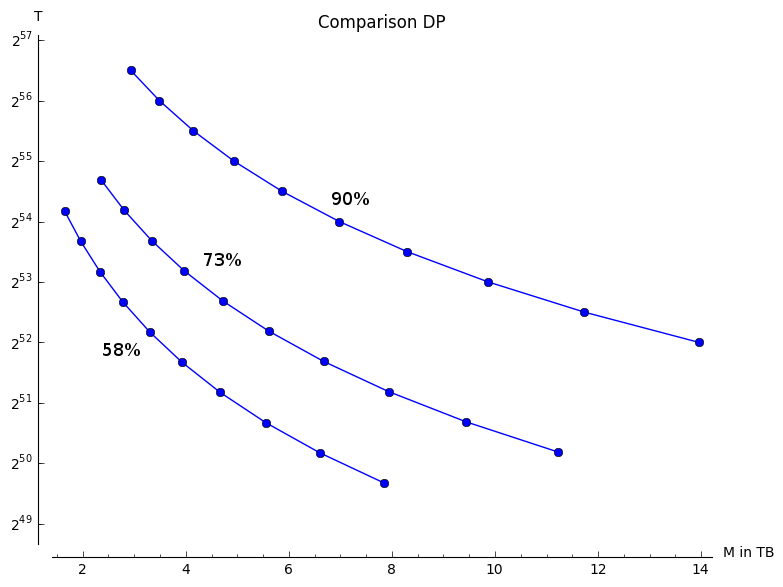
\includegraphics[scale=0.4]{figures/compareDP.png}
  \caption{Comparison of 58\%, 73\% and 90\% success TMTO}
  \label{fig:comparisonhell2.25}
\end{figure}



\section{Rainbow Table Parameters}
\label{sec:rainbowtab}
\begin{table}[h!]\centering
 \ \text{\texttt{Success{ }={ }0.540000,{ }Rmsc{ }={ }1.086067,{ }l{ }={ }1,{ }Offline{ }phase{ }={ }2{\char`\^}64.119113}}
\begin{tabular}{llll}
m & t & M(TB) & T \\ \hline
$2^{35.50}$ & $2^{28.42}$ & $0.39$ & $2^{55.61}$ \\
$2^{36.00}$ & $2^{27.92}$ & $0.55$ & $2^{54.61}$ \\
$2^{36.50}$ & $2^{27.42}$ & $0.78$ & $2^{53.61}$ \\
$2^{37.00}$ & $2^{26.92}$ & $1.10$ & $2^{52.61}$ \\
$2^{37.50}$ & $2^{26.42}$ & $1.55$ & $2^{51.61}$ \\
$2^{38.00}$ & $2^{25.92}$ & $2.20$ & $2^{50.61}$ \\
$2^{38.50}$ & $2^{25.42}$ & $3.11$ & $2^{49.61}$ \\
$2^{39.00}$ & $2^{24.92}$ & $4.40$ & $2^{48.61}$ \\
$2^{39.50}$ & $2^{24.42}$ & $6.22$ & $2^{47.61}$ \\
$2^{40.00}$ & $2^{23.92}$ & $8.80$ & $2^{46.61}$ \\
\end{tabular}
\end{table}


\begin{table}[h!]\centering
  \text{\texttt{Success{ }={ }0.900000,{ }Rmsc{ }={ }4.324555,{ }l{ }={ }1,{ }Offline{ }phase{ }={ }2{\char`\^}66.112552}}
  \begin{tabular}{llll}
    m & t & M(TB) & T \\ \hline
    $2^{35.50}$ & $2^{30.61}$ & $0.39$ & $2^{60.20}$ \\
    $2^{36.00}$ & $2^{30.11}$ & $0.55$ & $2^{59.20}$ \\
    $2^{36.50}$ & $2^{29.61}$ & $0.78$ & $2^{58.20}$ \\
    $2^{37.00}$ & $2^{29.11}$ & $1.10$ & $2^{57.20}$ \\
    $2^{37.50}$ & $2^{28.61}$ & $1.55$ & $2^{56.20}$ \\
    $2^{38.00}$ & $2^{28.11}$ & $2.20$ & $2^{55.20}$ \\
    $2^{38.50}$ & $2^{27.61}$ & $3.11$ & $2^{54.20}$ \\
    $2^{39.00}$ & $2^{27.11}$ & $4.40$ & $2^{53.20}$ \\
    $2^{39.50}$ & $2^{26.61}$ & $6.22$ & $2^{52.20}$ \\
    $2^{40.00}$ & $2^{26.11}$ & $8.80$ & $2^{51.20}$ \\
  \end{tabular}
\end{table}


\begin{table}[h!]\centering
  \text{\texttt{Success{ }={ }0.540000,{ }Rmsc{ }={ }0.311116,{ }l{ }={ }3,{ }Offline{ }phase{ }={ }2{\char`\^}63.900488}}
  \begin{tabular}{llll}
    m & t & M(TB) & T \\ \hline
    $2^{35.50}$ & $2^{26.64}$ & $1.17$ & $2^{52.18}$ \\
    $2^{36.00}$ & $2^{26.14}$ & $1.65$ & $2^{51.18}$ \\
    $2^{36.50}$ & $2^{25.64}$ & $2.33$ & $2^{50.18}$ \\
    $2^{37.00}$ & $2^{25.14}$ & $3.30$ & $2^{49.18}$ \\
    $2^{37.50}$ & $2^{24.64}$ & $4.66$ & $2^{48.18}$ \\
    $2^{38.00}$ & $2^{24.14}$ & $6.60$ & $2^{47.18}$ \\
    $2^{38.50}$ & $2^{23.64}$ & $9.33$ & $2^{46.18}$ \\
    $2^{39.00}$ & $2^{23.14}$ & $13.19$ & $2^{45.18}$ \\
    $2^{39.50}$ & $2^{22.64}$ & $18.66$ & $2^{44.18}$ \\
    $2^{40.00}$ & $2^{22.14}$ & $26.39$ & $2^{43.18}$ \\
  \end{tabular}
\end{table}

\begin{table}[h!]\centering
  \text{\texttt{Success{ }={ }0.730000,{ }Rmsc{ }={ }0.487727,{ }l{ }={ }3,{ }Offline{ }phase{ }={ }2{\char`\^}64.549108}}
  \begin{tabular}{llll}
    m & t & M(TB) & T \\ \hline
    $2^{35.50}$ & $2^{27.46}$ & $1.17$ & $2^{53.76}$ \\
    $2^{36.00}$ & $2^{26.96}$ & $1.65$ & $2^{52.76}$ \\
    $2^{36.50}$ & $2^{26.46}$ & $2.33$ & $2^{51.76}$ \\
    $2^{37.00}$ & $2^{25.96}$ & $3.30$ & $2^{50.76}$ \\
    $2^{37.50}$ & $2^{25.46}$ & $4.66$ & $2^{49.76}$ \\
    $2^{38.00}$ & $2^{24.96}$ & $6.60$ & $2^{48.76}$ \\
    $2^{38.50}$ & $2^{24.46}$ & $9.33$ & $2^{47.76}$ \\
    $2^{39.00}$ & $2^{23.96}$ & $13.19$ & $2^{46.76}$ \\
    $2^{39.50}$ & $2^{23.46}$ & $18.66$ & $2^{45.76}$ \\
    $2^{40.00}$ & $2^{22.96}$ & $26.39$ & $2^{44.76}$ \\
  \end{tabular}
\end{table}

\begin{table}[h!]\centering
  \text{\texttt{Success{ }={ }0.900000,{ }Rmsc{ }={ }0.935599,{ }l{ }={ }3,{ }Offline{ }phase{ }={ }2{\char`\^}65.488924}}
  \begin{tabular}{llll}
    m & t & M(TB) & T \\ \hline
    $2^{35.50}$ & $2^{28.40}$ & $1.17$ & $2^{55.57}$ \\
    $2^{36.00}$ & $2^{27.90}$ & $1.65$ & $2^{54.57}$ \\
    $2^{36.50}$ & $2^{27.40}$ & $2.33$ & $2^{53.57}$ \\
    $2^{37.00}$ & $2^{26.90}$ & $3.30$ & $2^{52.57}$ \\
    $2^{37.50}$ & $2^{26.40}$ & $4.66$ & $2^{51.57}$ \\
    $2^{38.00}$ & $2^{25.90}$ & $6.60$ & $2^{50.57}$ \\
    $2^{38.50}$ & $2^{25.40}$ & $9.33$ & $2^{49.57}$ \\
    $2^{39.00}$ & $2^{24.90}$ & $13.19$ & $2^{48.57}$ \\
    $2^{39.50}$ & $2^{24.40}$ & $18.66$ & $2^{47.57}$ \\
    $2^{40.00}$ & $2^{23.90}$ & $26.39$ & $2^{46.57}$ \\
  \end{tabular}
\end{table}
\section{Rainbow Table Graphs}
\label{sec:rainbowgraphs}
\begin{figure}[H]
  \centering
  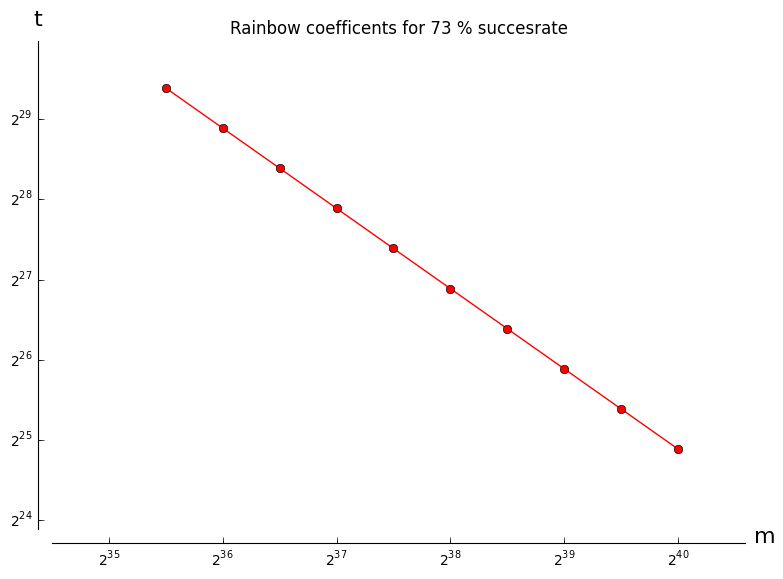
\includegraphics[scale=0.5]{figures/RainbowCoef73.png}
  \caption{Rainbow Parameters for 73\% success}
\end{figure}

\begin{figure}[H]
  \centering
  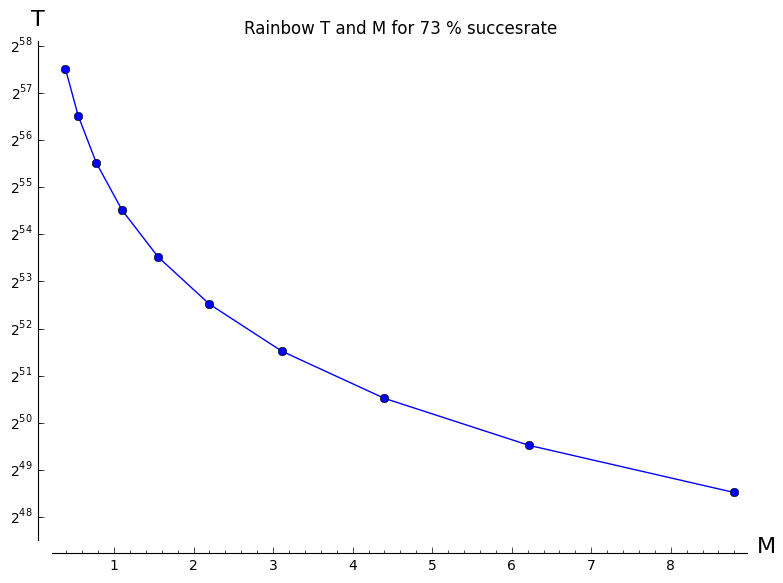
\includegraphics[scale=0.5]{figures/RainbowTime73.png}
  \caption{Rainbow TMTO for 73\% success}

\end{figure}

\begin{figure}[H]
  \centering
  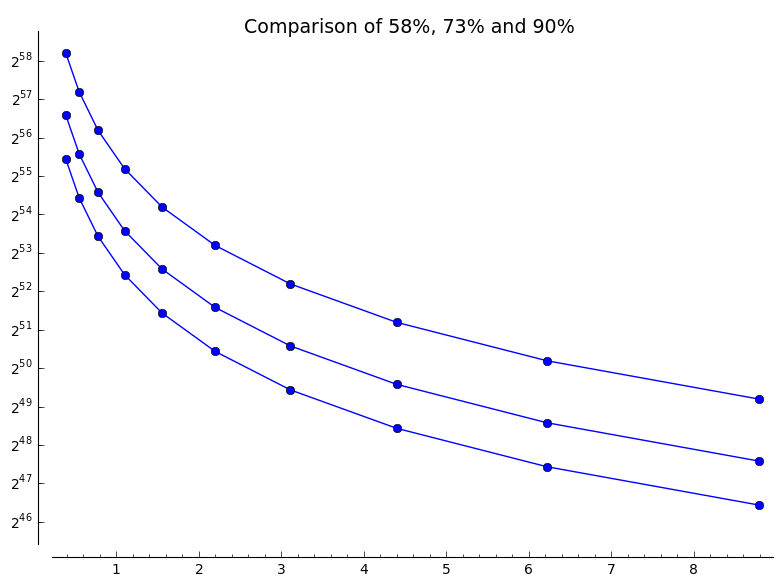
\includegraphics[scale=0.4]{figures/RainbowAllCalc.png}
  \caption{Comparison of 58\%, 73\% and 90\% success TMTO}
  \label{fig:comparisonrain}
\end{figure}

%%% Local Variables:
%%% mode: latex
%%% TeX-master: "Thesis"
%%% End:

%-----------
% Backmatter
%-----------
\nocite{176}
\nocite{DP}
\nocite{sand}
\nocite{single}
\nocite{rect}
\nocite{relate}
\nocite{diff}
\nocite{single2002}
\nocite{imp}
\nocite{rectangle}
\nocite{boom}
\nocite{nohl}
\backmatter
\chaptermark{Bibliography}
\renewcommand{\sectionmark}[1]{\markright{#1}}
\sectionmark{Bibliography}
\addcontentsline{toc}{chapter}{Bibliography}        %Force addition of Bibliography to TOC
\bibliographystyle{alpha}                           %Use alpha codes for references
\bibliography{References}                           %Bibliography file called
\end{document}
% % % EOF % % %
%%% Local Variables:
%%% mode: latex
%%% TeX-master: t
%%% End:
